\DontNumberThisInToc
\DontFrameThisInToc
\glsresetall
\ChapterNumberCitation{La sélection de l'action émerge de la topologie intrinsèque: un modèle du colliculus supérieur}{The brain is one of the most complex systems in nature, with a structured complex connectivity. Recently, large-scale corticocortical connectivities, both structural and functional, have received a great deal of research attention, especially using the approach of complex network analysis. Understanding the relationship between structural and functional connectivity is of crucial importance in neuroscience}{Changsong Zhou et al 2007 New J. Phys. 9 178 }{10cm}

\section{Introduction}

Le colliculus supérieur [\gls{sc}] est une structure multimodale du tronc cérébral impliquée dans plusieurs fonctions cérébrales complexes. Cette structure sous-corticale a été intensivement étudiée, tant au niveau structurel qu'au niveau fonctionnel. Il s'agit d'une structure laminaire. Ses couches superficielles (I, II \& III) sont connues pour recevoir des entrées principalement de la rétine, les cortex visuels primaires [\gls{v1}] et secondaires [\gls{v2}] et les champs oculaires frontaux [\gls{fef}] tandis que les couches intermédiaires (IV \& V) et les couches profondes (VI \& VII) reçoivent la contribution de plusieurs aires sensorielles et motrices ainsi que des noyaux gris centraux [\gls{bg}] \cite{May:2006,McHaffie:2005}. L'activation endogène ou exogène de ces couches profondes peut déclencher le mouvement des yeux. La fonction du colliculus supérieur a été largement étudiée au cours des 40 dernières années grâce à une série d'expériences intéressantes (\cite{Levy-Schoen:1969, Robinson:1972, Sparks:1976, Sparks:1980, Lee:1988, Munoz:1995a, Anderson:1998, Badler:2002}) qui a éclairé le rôle crucial du colliculus supérieur dans le contrôle des mouvements oculaires tels que la fixation, la poursuite lisse, les saccades et les mouvements de vergence.\\

\begin{figure*}[htbp!]
  \centering
    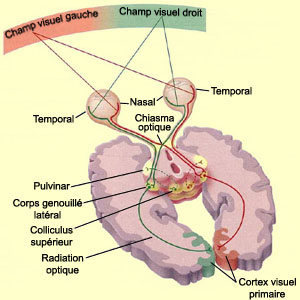
\includegraphics[width=0.4\textwidth]{figures/ch3_1_colliculus}\\

  \caption{ Position des deux colliculus dans le circuit visuo-moteur.}
  \label{fig: coll}
\end{figure*}

Afin d'éclaicir les mécanismes assurant la corrélation entre cette structure du cerveau et sa fonction visuo-motrice, plusieurs modèles du \gls{sc} ont été proposés  \cite{VanGisbergen:1985, Scudder:1988, Droulez:1991, Arai:1994,Nichols:1995, Breznen:1997, Lefevre:1998, Findlay:1999, Gancarz:1999, Short:2001, Trappenberg:2001, Badler:2002, Goossens:2006, Nakahara:2006, Marino:2008, Marino:2012} permettant de simuler numériquement plusieurs caractéristiques du comportement visuo-moteur et de ses circuits neuronaux fondamentaux.\\


La plupart de ces modèles ont été conçus pour aborder des questions spécifiques (comportement ou proprieté) basées sur différents mécanismes et jusqu'à aujourd'hui il reste très difficile d'avoir une vision synthétique qui caractérise clairement la contribution du \gls{sc} à la génération des saccades visuelles aussi bien au niveau électrophysiologique qu'au niveau comportemental. Un modèle complet  comprenant tous ces mécanismes pourrait peut être entièrement expliquer comment cette structure contribue à la génération des saccades mais assembler ces modèles est hors de portée parce qu'ils ne sont, pour la plupart, pas compatibles les uns avec les autres. Ils sont fondés sur différentes hypothèses liées à l'architecture, aux afférences ou aux caractéristiques fonctionnelles pour expliquer les mêmes phénomènes.\\

Nous avons donc décidé d'identifier les caractéristiques communes à ces modèles pour établir une proposition d'un modèle minimaliste. Ce modèle prend en compte les proprietés de base bien reconnues, principalement la représentation log-polaire de la surface rétinienne dans les couches profondes du \gls{sc} \cite{Ottes:1986}, le profil de connectivité latérale dans le \gls{sc} et la dynamique de l'activité de neurones colliculaires. Le modèle résultant est inévitablement beaucoup plus simple que les autres modèles déjà proposés. Cependant, nous rapportons un grand ensemble de résultats que nous avons pu reproduire et qui ont été souvent exploités pour valider des modèles beaucoup plus complexes. Nous proposons ici que des hypothèses plus simples sont suffisantes pour expliquer ces résultats et que beaucoup de propriétés émergent simplement des caractéristiques locales et bien connues.\\
%%%%%%%%%%%%%%%%%%%

Nous allons d'abord passer en revue quelques modèles déjà existants pour détailler ensuite les hypothèses que nous avons retenues. Sur la base de ces hypothèses, nous présentons dans la section des résultats un certain nombre de propriétés émergentes telles que le codage par population, la latence des saccades et la reproduction d'autres observations classiques électrophysiologiques et comportementales. En particulier, ce modèle offre un paradigme de sélection basé uniquement sur l'architecture intrinsèque. Enfin nous discuterons les principaux résultats de cette approche de modélisation.\\
%%%%%%%%%%%%%%%%%%%%%%%%%%%%%%%%%%%%%%%%%%%%%%%%%%%%%%%%%%%%%%%%%%%%%%%%%%%%%%%%%%%%%%%%%%%%%%%%%%%%%%%%%%

\section{Modèles de colliculus}

Chez les mammifères, le \gls{sc} est considéré comme une structure clé impliquée dans l'attention visuelle et le déclenchement de saccades \cite{Isa:2002}. D'une part, le \gls{sc} a été d'abord décrit comme une interface de transformation de signaux sensoriels en commandes motrices. Il reçoit les signaux rétiniens dans ses couches superficielles et renvoie à travers ses couches profondes prémotrices des ordres vers la formation réticulée [\gls{rf}]. D'autre part, cette structure participe également à des comportements plus complexes qui impliquent la sélection des cibles potentielles sur la base de facteurs exogènes et endogènes \cite {Kramer:1999}. Le \gls{sc} est donc considéré comme une importante structure d'intégration visuo-motrice. De nombreux modèles ont étudié ses propriétés physiologiques et comportementales (voir \cite {Girard:2005} pour une revue), ainsi que les différents flux d'information impliquant les couches colliculaires.  \\

\subsection{Intégration sensorimotrice}

Le colliculus supérieur agit comme un site d'intégration sensorimotrice, en recevant, entre autres, des entrées somato-sensorielles, auditives, ainsi que des signaux visuels\cite{Nolte:1993}. Ses entrées visuelles arrivent, soit directement de la rétine, soit par l'intermédiaire du cortex (modulées par l'intervention d'autres structures), pour fournir en sortie des prévisions des déplacements désirés à transmettre aux muscles oculaires via les neurones moteurs\cite{Wurtz:1996,Nolte:1993,Ursino:2009}. \\

En effet, la couche superficielle du colliculus supérieur est une couche visuelle qui reçoit des informations directement des cellules ganglionnaires de la rétine. Chaque site de cette couche s'active de façon optimale pour un stimulus présent en un point particulier du champ visuel. De son côté, la couche profonde forme une carte motrice topographiquement organisée : les vecteurs de la saccade résultante d'un stimulus visuel varient selon la position du stimulus. La correspondance entre les deux cartes fait penser à un mécanisme simple pour guider les yeux: un stimulus visuel projeté sur la rétine entraîne l'activation de la carte visuelle qui excite directement la carte motrice qui à son tour prépare l'ordre moteur permettant le déplacement désiré.\\

Ce modèle simple a été proposé dès 1970 suite à la découverte des cartes colliculaires. A l'époque, il était difficile de prouver l'existence des connexions descendantes directes entres les couches et de plus, il a été montré que les saccades n'exigent pas l'existence d'un stimulus visuel (saccades spontanées dans l'obscurité). Par la suite, ce modèle a été restreint aux saccades réflexes à très courte latence (saccades express) après avoir montré l'existence d'une connexion anatomique directe. Pour les saccades à plus grande latence, les chercheurs se sont dirigés vers des modèles qui intègrent des voies indirectes en passant par le cortex et les structures sous-corticales\cite{Wurtz:1996,Purves:2005}.\\ 

La structure du modèle décrit dans \cite {Findlay:1999} souligne que la principale tâche est de décider quand et où la saccade doit être effectuée. En conséquence, deux axes hiérarchiques sont définis. L'axe ``quand?'' (correspondant à \gls{fef}) décide du moment de quitter le point de fixation courant, alors que l'axe ``o\`u'' (correspondant au \gls{sc}) met en œuvre une compétition spatiale entre les cibles candidates. Un modèle combinant le \gls{fef} et le \gls{sc} a également été proposé dans \cite {Kramer:1999}, pour expliquer l'intégration d'éléments exogènes (stimuli externes en provenance de la rétine et des éléments endogènes (internes ou consignes élaborées dans le cortex préfrontal). \\

Plus tard, \cite {Godijn:2002} ont proposé un modèle computationnel d'intégration fondée sur de solides preuves expérimentales au niveau comportemental, qui suppose que tous ces éléments (traitement spatial, traitement temporel, stimuli exogènes et stimuli endogènes) peuvent être intégrés dans une seule carte, considérée comme un modèle du \gls{sc}. Il décrit donc le \gls{sc} comme une structure multimodale.\\

Cette carte inclut également des propriétés généralement considérées comme physiologiquement plausible: une excitation locale permettant de combiner des stimuli proches et un mécanisme d'inhibition plus large permettant de déclencher une compétition entre les stimuli éloignés \cite {VanOpstal:1989, Tweed:1990, Munoz:1998}. Ce schéma d'interaction explique pourquoi il a été possible d'utiliser un formalisme de champs neuronaux dynamiques [\gls{dnf}] \cite {Amari:1977} utilisé aussi dans \cite {Trappenberg:2001, Schneider:2002, Badler:2002,Marino:2012}. \\


D'autres études plus spécifiques proposent des éléments de la connectivité intrinsèque, afférente et efférente du \gls{sc}. C'est par exemple le cas pour la définition de plusieurs types de comportements neuronaux liés à différentes étapes de sélection de la cible \cite{Wurtz:1994} (\ref{typ}) et l'impact de la rétinotopie de projections visuelles sur la nature du traitement colliculaire \cite{Trappenberg:2001, Schneider:2002,Godijn:2002} (\ref{retin}) pour permettre d'évaluer le rôle de l'activité colliculaire dans l'encodage des saccades (\ref{eval}).




\subsection{Typologie neuronale}{\label{typ}}

La typologie des neurones colliculaires a été largement étudiée \cite {Wurtz:1994, Moschovakis:1996}. Il en résulte de nombreux modèles du colliculus supérieur sur des populations hétérogènes de neurones avec des dynamiques complexes. La plupart des modèles récents donnent un rôle plus important au \gls{sc} au prix d'un fonctionnement interne plus complexe. En effet, ces modèles définissent plusieurs types d'unités, en fonction de leur emplacement sur la carte, ce qui n'est pas très compatible avec le principe d'homogénéité dans les \glspl{dnf}. Wurtz et Optican ont proposé un modèle du \gls{sc} organisé en modules verticaux selon trois classes de neurones \cite{Wurtz:1994} : les neurones de fixation (FN), les neurones \textit{burst} (BN) et les neurones \textit{build-up} (BUN). La classification est faite en se basant sur des critères décrits précédemment dans \cite {Goldberg:1972,Munoz:1993a,Dorris:1997,Munoz:1995a}. \\



Par exemple, pour être classé comme un build-up, un neurone doit être situé entre 1 à 3 mm au-dessous de la surface dorsale du colliculus supérieur, doit commencer à décharger à une faible fréquence après le signal de déclenchement d'une saccade et doit continuer sa décharge jusqu'à la fin de la saccade \cite{Munoz:1995a,Dorris:1997}. \\



Cette classification reste une hypothèse permettant de définir plusieurs modèles de contrôle saccadique \cite{Trappenberg:2001, Schneider:2002}. Dans \cite {Godijn:2002} aussi, le substrat de calcul n'est pas homogène car la sensibilité des unités diminue avec leur excentricité sur la carte. Cette astuce est utilisée pour reproduire l'observation que la latence d'une saccade vers une cible, présentée conjointement avec un élément de distraction, est plus longue lorsque le distracteur est plus proche de la zone rostrale du \gls{sc} (correspondant à la fovéa).\\ 

Mais certains chercheurs optent plutôt pour une seule population homogène de cellules colliculaires qui change de comportement en fonction des paramètres extérieurs et des conditions expérimentales \cite {Trappenberg:2001, Droulez:1991}. Certaines études défendent l'existence d'une continuité entre les neurones de fixations et les autres neurones (appelés ``neurones de saccades'') \cite{Munoz:1995a}.\\


\subsection{Carte colliculaire topographique} {\label{retin}}

Les relations de voisinage spatial que les cellules ganglionnaires entretiennent entre elles au sein de la rétine, sont préservées au niveau de leurs cibles  corticales et sous-corticales. Les structures visuelles centrales présentent donc une représentation ordonnée de l'espace visuel \cite{Purves:2004}.\\

Au sein des aires visuelles primaires, la fovéa est représentée proche du pôle occipital, alors que les régions périphériques sont projetées sur les parties plus antérieures de la surface corticale. Les projections des excentricités sont donc encodées dans la direction postéro-antérieure (rostro-caudale). En outre, la carte rétinotopique est souvent déformée, ceci est lié au fait que l'espace visuel n'est pas uniformément échantillonné au niveau de la rétine.\\

Pour analyser la rétinotopie de manière quantitative, les modélisateurs définissent un système de coordonnées dans le champ visuel. Les coordonnées les plus adaptées au système visuel sont les coordonnées polaires $(\rho,\phi)$. On caractérise alors une position dans le champ visuel par son excentricité $\rho$ par rapport au centre du regard et par son angle polaire $\phi$, mesuré par exemple par rapport au méridien vertical inférieur. \\

Ensuite une carte rétinotopique est souvent approchée par une transformée log-polaire de l'image rétinienne \cite{Robinson:1972}. Le modèle le plus utilisé pour effectuer la transformation des coordonnées polaires du stimulus visuel sur la rétine en coordonnées cartésiennes sur le colliculus supérieur est celui proposé par \cite{Ottes:1986}.\\

Il s'agit d'un modèle quantitatif de la structure des cartes colliculaires basé sur la cartographie (mapping) obtenue expérimentalement par \cite{Robinson:1972} en stimulant électriquement le colliculus chez le singe. Il propose une fonction de projection logarithmique qui assure la projection des coordonnées rétiniennes en coordonnées colliculaires. Les équations de cartographie résultantes ont été ensuite utilisées dans plusieurs modèles \cite {VanGisbergen:1987,Optican:1995, Trappenberg:2001, Lefevre:1998, Marino:2008, Nakahara:2006}.\\
%En utilisant ce modèle, la rétine peut être réduite à la couche de photo-récepteurs.  

\subsection{\'Evaluation de l'activité colliculaire} {\label{eval}}

La plupart des modèles de génération de saccades supposent que les trajectoires des saccades sont stéréotypées. La vitesse et l'amplitude des saccades sont déterminées par l'activation d'une sous-population de neurones du colliculus supérieur profond \cite{Sparks:1990}. Mais des données expérimentales ont montré que les saccades ont des trajectoires assez variables \cite {Erkelens:1995}. Dans ces modèles de générateurs de saccades, différentes hypothèses ont été faites sur la nature des signaux codés au sein de l'activité colliculaire, i.e. la taille de la saccade désirée ou l'erreur motrice \cite{Waitzman:1988}. \\
%%%MOving hill"

Plusieurs modèles basés principalement sur des expériences sur le chat, supposent que les saccades sont initiées par une activité neuronale colliculaire qui se déplace au cours de la saccade de la zone caudale (périphérique) vers la zone rostrale (fovéale). Le but est d'amener l'activité résultant d'une stimulation vers la zone de fixation correspondant à la projection de la zone fovéale \cite {Droulez:1991, Lefevre:1992, Optican:1994 , Massonne:1994, Wurtz:1994, Schierwagen:1996, Grossberg:1997}. Cette hypothèse n'est plus supporté, certaines études sur les singes ont montré l'inexistence de cette translation d'activité \cite{Robijanto:2002}. L'activité neuronale pendant les saccades est plutôt considérée stationnaire et stéréotypée comme spécifié dans \cite {Anderson:1998}.\\
%%%%SStériotypée

Le modèle proposé dans \cite{VanOpstal:2008} suppose que la forme et la taille de la sous-population colliculaire activée par un stimulus visuel sont invariantes pour toutes les saccades et que cette sous-population active peut être décrite par un profil gaussien d'une largeur fixe et un maximum de fréquence moyenne de décharge. Ce modèle récent est basée sur une formulation mathématique et produit des résultats satisfaisants, mais il n'aide pas à comprendre la structure du colliculus supérieur et des connexions possibles incluses dans le contrôle du regard. Il s'agit d'imposer certaines propriétés qui sont censées être des fonctions émergentes, c'est pourquoi des modèles computationnels à base de réseaux neurones nous semblent plus appropriés à la compréhension du lien entre la structure et ses fonctions.\\
%%%décodage

De nombreux schémas de décodage de l'activation colliculaire ont été proposés \cite {McIlwain:1976, Sparks:1976, Massonne:1994, Badler:2002, Lee:1988, Bozis:1998}. Plusieurs schémas d'évaluation de la sortie du \gls{sc} ont été proposés. Le schéma le plus simple est celui du \textit{winner-takes-all} où le site le plus actif impose la direction, en supposant que chaque site code pour une direction. Ensuite, deux schémas de calcul sont souvent proposés dans les modèles de décodage de l'activité colliculaire:\\

\begin{itemize}

\item le vecteur moyenne \cite {Lee:1988} basé sur une normalisation qui dépend du nombre de neurones actifs. Dans ce schéma de décodage, on parle plutôt de la ``contribution'' $\vec{R}_n$ d'une cellule $n$ au vecteur de mouvement (déplacement) \cite{Walton:2005, Lee:1988}. La somme correspond donc à l'addition des contributions de toutes les cellules de la population. Le vecteur déplacement $\vec{S}$ vers la cible de la saccade est calculé en fonction des fréquences de décharges moyennes $r_n$ comme suit:

\begin{align}
  \vec{S} = \frac{\sum_{n=1}^{N} r_n\vec{R}_n }{\sum_{n=1}^{N} r_n}
\label{moy}
\end{align} 

\item le vecteur somme \cite{McIlwain:1976, Sparks:1976} où toutes les activités des neurones colliculaires sont additionnées avec des pondérations fixées selon la position sur la carte. Dans ce schéma de décodage, on désigne une ``direction préférée'' pour chaque cellule. Plus généralement, à chaque cellule correspond un champ de mouvement qui correspond à l'ensemble des directions pour lesquelles cette cellule s'active. Si on utilise le décodage par somme, il faut définir la contribution de chaque cellule dans le mouvement définie comme l'amplitude caractéristique divisée par la taille de la bulle d'activité. Cette bulle d'activité est supposée avoir une amplitude constante indépendamment de sa position. La contribution $\vec{m}_n$ d'un neurone $n$ est une grandeur caractéristique du neurone indépendante de son activation. Le vecteur déplacement est calculé comme suit: 

\begin{align}
  \vec{S} = \sum_{n=1}^{N} r_n\vec{m}_n 
\label{moy}
\end{align} 

\end {itemize}

\begin{figure}[ht]
  \begin{center}
    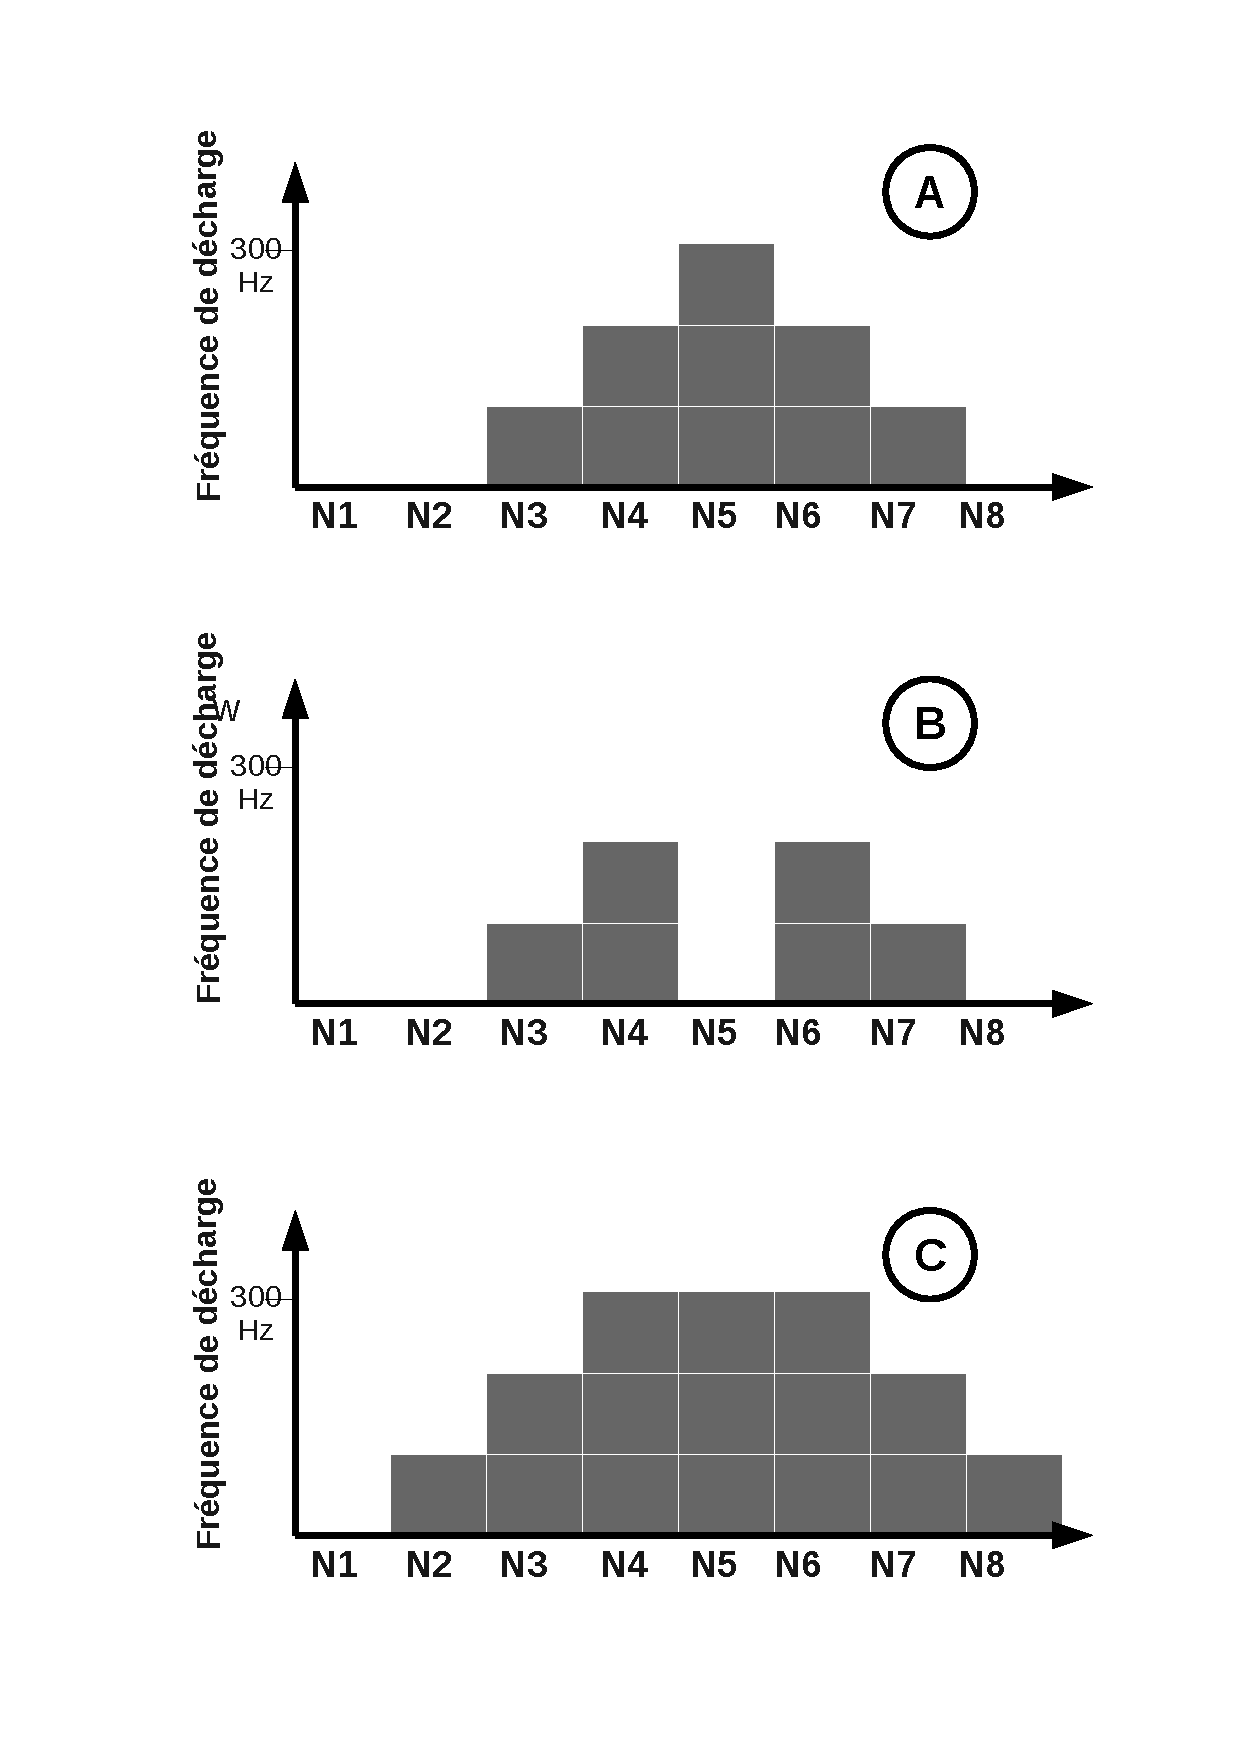
\includegraphics[width=0.6\textwidth,height=10cm]{figures/ch3_2_sum-average}
  \end{center}
  \caption{ Exemple théorique illustrant la différence entre les schémas de décodage de l'activation colliculaire sur une carte supposée linéaire: A- Cas normal, B- Inhibition partielle de la zone active C- Sur-activation. Les diagrammes correspondent aux fréquences de décharge d'une population de neurones $Ni$, $i\protect\in[1..8]$, en prenant en compte leur disposition spatiale. Les neurones N4 et N6 sont par exemple les voisins immédiats du neurone N5.}
  \label{sumav}
\end{figure}

Considérons un exemple simple illustré par la figure (fig.\ref{sumav}-A). On considère que la direction préférentielle d'un neurone $N_i$ se situe à une amplitude $i$. Le neurone N5 étant le plus activé, s'il décide tout seul, la saccade correspondant à ce profil d'activation serait d'une amplitude de 5°. Le décodage par moyenne et le décodage par somme donnent la même valeur (5) dans le cas normal\footnote{
\textit{L'amplitude désirée selon le décodage par moyenne}\\
\textit{= la somme des directions pondérées par les activations/ somme totale des activations }\\
                     $=(0+0+100*3+200*4+300*5+200*6+100*7+0)/(100+200+300+200+100)=5$\\

Si on considère un décodage par somme, on définit les contributions des neurones. La contribution du neurone N2, par exemple, $vaut 2/900=0.00222$. La contribution du neurone N2, par exemple, $vaut 2/900=0.00222$. D'o\`u:\\

\textit{L'amplitude désirée selon le décodage par somme}\\
\textit{= la somme des contributions des cellules de la population active pondérée par leurs activations}\\
                     $=(0+0+100*3/900+200*4/900+300*5/900+200*6/900+100*7/900+0)=5$\\}.\\

Ces deux modes d'évaluation sont équivalents dans le cas d'une population saine activée normalement (pas de lésions) mais peuvent différer en cas d'inactivation (par injection de substances inhibitrices par exemple) ou de sur-activation (par stimulation électrique par exemple). Prenons les cas illustrés par les figures (fig.\ref{sumav}-B, fig.\ref{sumav}-C).\\

La figure B correspond à une lésion, le calcul de la moyenne donne une amplitude de $5$ mais le calcul de la somme donne une amplitude de $3.33$. De même dans le cas d'une sur-activation, la figure C, les résultats ne sont pas convergents, avec le vecteur somme on obtient $8.33$ et avec le vecteur moyenne on obtient $5$.\\

Ces schémas sont considérés d'un point de vue ``statique'' en supposant que le colliculus supérieur n'est pas inclus dans la boucle de feedback moteur contrairement à ce que proposent plusieurs modèles \cite{Robinson:1972}. L'activité du colliculus est supposée coder le déplacement désiré et non-pas l'erreur motrice instantanée (ce qui reste à l'oeil à parcourir pour arriver au but). \cite{Gandhi:2011} introduisent un troisième schéma qui décode l'activité au fur et à mesure que l'activité évolue qu'on ne détaillera pas ici.\\

Certaines expériences ont donné des résultats en faveur de la moyenne \cite{Lee:1988}, d'autres plutôt en faveur de la somme sans donner une synthèse concluante. Le problème est que ces expériences restent compliquées et non maîtrisées (le dosage, la diffusion, la précision de l'injection, les neurones affectés...) et difficilement reproductibles.\\

Nous détaillerons dans la section suivante les hypothèses que nous avons retenues de tous ces modèles pour proposer un modèle minimaliste permettant de reproduire et d'expliquer un certain nombre de résultats d'expériences biologiques décrits et discutés dans la suite.\\
%\subsection{Synthèse}
%{\scriptsize
%\begin{tabular}{|c|c|c|c|c|c|c|c|c|}
%\hline
%	& {\em Connectivité} & {\em Typologie} &{\em Mapping }&{\em Entrées}& {\em Sorties }& {\em Fonctions}\\
%	& {\em latérale}  & {\em neuronale}  &        {\em }&{\em Stimulus}& {\em Décodage }& {\em Dynamique}\\
%\hline
%\cite{Tabareau:2006}&           &	BN/BUN	&    linéaire             &			&           somme pondérée      & seulment BN 		\\
%&           &		&    ou log            &			&                 &	activité stéréotypée	\\
%\hline
%\cite{Stephan:2002}	&   inhib+excit & BUN   &                 &			&                 &	accumulation BUN \\

%	&                 &		BN &                &			&                 &	sélection BN		\\

%	&                 &		FN   &             &			&                 &		\\
%\hline
%\cite{Lee:1988}	&                 &		&                 &			&       vector sum           &		\\
%&                 &		&                 &			&      by ihibition          &		\\
%\hline
%\cite{Badler:2000}	&                 &		&                 &			& vector avg               &		\\
%\hline
%\cite{Anderson:1998}	& &   BUN/BN              &	log-polaire	                &			&                 &		\\
%\hline
%\cite{Wurtz:1994}	&                 & BUN/BN/FN	&                 &			&                 &stationnaire		\\%
%	&                 &		&                 &			&                 &/mouvante		\\
%\hline
%\cite{Opstal:2008}	&                 &		&                 &			&                 &	Math stéréotypée	\\
%\hline
%\cite{Goossens:2008}	&    non             &	non	&                 &	gaussienne		&    vector sum             &		\\
%\hline
%\end{tabular}
%}
%%%%%%%%%%%%%%%%%%%%%%%%%%%%%%%%%%%%%%%%%%%%%%%%%%%%%%%%%%%%%%%%%%%%%%%%%%%%%%%%%%%%%%%%%%%%%%%%%%%%%%%%%%%%%%%%%%%%%%%%%%%%%%%%%%%%%%%%%%%%%%%%%%%%%%%%%%%%%%%%%%%%%%%%%%%%%%%%%%%%
\section{Hypothèses et méthodes}

Nous avons simulé numériquement un modèle de réseau de neurones de trois couches organisées topologiquement en utilisant le formalisme de \textit{champs neuronaux dynamiques} [\gls{dnf}] décrit dans le premier chapitre \cite{Amari:1977}. La première couche correspond à la rétine et la deuxième couche correspond au colliculus supérieur profond. Une troisième couche intermédiaire est aussi utilisée qui peut représenter des structures intermédiaires telles que \gls{v1} et qui servira principalement à expliciter la déformation log-polaire (décrite dans la suite) de la projection de la carte rétinienne sur la carte colliculaire. D'un point de vue numérique, cette couche intermédiaire n'est pas indispensable, la projection peut se faire directement sur la carte colliculaire. Comme expliqué dans l'introduction, le modèle a été établi seulement sur la base des hypothèses communes à d'autres modèles du \gls{sc} que nous résumons dans les cinq points suivants:\\

\begin{itemize}

\item[$\bullet$] Un stimulus physique (une cible) est représenté sur la surface (correspondant à la rétine) par une petite activation gaussienne (à deux dimensions). La rétine est réduite donc à une couche de photorécepteurs et nous considérons que le niveau de l'activation de ces récepteurs est proportionnel à l'intensité de la lumière.\\

\item[$\bullet$] On suppose que le lieu de l'activation sur le \gls{sc} code l'emplacement de la cible dans le champ visuel et que cette activation est à l'origine de la saccade qui apportera l'image de la cible sur la fovéa (fovéation). Deux activations voisines dans la couche \gls{sc} correspondent à des localisations de cibles voisines dans le champ visuel (codage topographique) \cite{Schiller:1972, Wurtz:1972}.\\

\item[$\bullet$] La projection du champ visuel sur la surface colliculaire est basée sur le modèle quantitatif de \cite{Ottes:1986} qui propose qu'une fonction de cartographie logarithmique assure la transformation des coordonnées rétiniennes en coordonnées colliculaires (une projection log-polaire). Nous supposons également que le stimulus est projeté en entier sur le \gls{sc} et non pas seulement son centre de masse.\\

\item[$\bullet$] Nous considérons le colliculus supérieur comme étant une carte homogène et uniforme d'unités neurales \cite{Trappenberg:2001,Droulez:1991}. En plus de ses afférences rétiniennes excitatrices, d'autres entrées excitatrices et inhibitrices latérales intracolliculaires qui dépendent de la distance entre les neurones sont considérées, comme proposé dans beaucoup de modèles \cite{Arai:1994, Droulez:1991, Gancarz:1999, Lefevre:1992, Optican:1995, Short:2001, Trappenberg:2001, Nakahara:2006}.\\

\item[$\bullet$] Les influences des aires corticales, des ganglions de la base et du cervelet sur l'activité colliculaire ne sont pas considérées ici.(sauf que l'inhibition latérale pourrait correspondre à une entrée inhibitrice de \gls{bg} (\gls{gpi}), comme proposé dans plusieurs papiers \cite{Trappenberg:2001})\\

\item[$\bullet$] Un seul colliculus est considéré.\\
\end{itemize}
L'architecture globale du modèle est donnée par la figure \ref{archi}.
\begin{figure}[ht]
  \begin{center}
    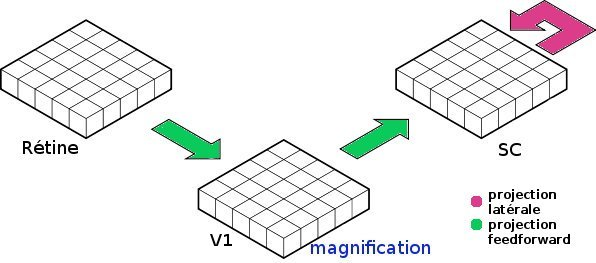
\includegraphics[width=0.7\textwidth]{figures/ch3_3_model0}
  \end{center}
  \caption{ Architecture du modèle. Une carte d'entrée représentant une demi rétine. Une carte intermédiaire (V1) représentant la projection rétinotopique. Une carte de sortie représentant la couche pré-motrice du colliculus supérieur }
  \label{archi}
\end{figure}
\subsection{L'entrée rétinienne}

 L'hémichamp visuel $V$ $[0^\circ,90^\circ]\times[-90^\circ,90^\circ]$ est projeté sur l'espace continu $R$ $[0,1]\times[-1,1]$ correspondant à la moitié d'une rétine. N'importe quel stimulus $S$ présenté dans $V$ aux coordonnées polaires $(\rho_s,\phi_s)$ (en degrés) est projeté sur $R$ aux coordonnées cartésiennes $(u_s, v_s)$. Nous avons considéré des stimuli ronds avec une distribution gaussienne de la luminosité tels que l'activité $U_r (u, v)$ en un point $(u, v)$ de $R$ en présence d'un stimulus S est donnée par l'équation suivante :\\

\begin{align}
  U_r(u,v)= C~exp\left(-\frac{\vert u - u_s\vert^2 + \vert v - v_s \vert^2}{2{\sigma_c}^2}\right)
\end{align}

en supposant que $(u_s, v_s)$ est le centre de la projection du stimulus sur la carte R, $\sigma_c$ est la taille angulaire du stimulus et $C$ est l'activation maximale dans $R$ (correspondant à l'intensité maximale du stimulus). Les stimulus sont supposés avoir approximativement un diamètre angulaire de 1° dans la rétine, qui correspond à $\sigma_c=1/90$.\\

\subsection{La projection visuelle sur le colliculus supérieur profond }

Selon la description de \cite{Robinson:1972}, la projection de $R$ sur le \gls{sc} est approximée en utilisant une transformation log-polaire, qui réduit le modèle de \gls{sc} à une carte bi-dimensionnelle. Une approximation mathématique de cette transformation a été proposée par \cite{Ottes:1986}. Il s'agit de la projection standard utilisée dans la plupart des modèles computationnels du colliculus \cite{Optican:1995, Trappenberg:2001, Lefevre:1998, Marino:2008, Nakahara:2006} :

\begin{align}
  x &=
  B_x~log\left(\frac{\sqrt{\rho^{2}+2A\rho|\cos{(\phi)}|+A^{2}}}{A}\right) \notag \\
  y &=
  B_y~arctan\left(\frac{\rho \sin{(\phi)}}{\rho|\cos{(\phi)}|+A}\right)
  \label{eq: mapping}
\end{align}

où $(x,y)$ représentent les coordonnées cartésiennes dans le \gls{sc} (en millimètres), $(\rho,\phi)$ les coordonnées polaires dans $R$ (en degrés). $Bx$ (en millimètres) est une constante déterminant la taille de la carte colliculaire le long de l'axe horizontal. $By$ (en millimètres) est une constante déterminant la taille de la carte colliculaire le long de l'axe vertical. $A$ (en degrés) est une constante qui (avec le rapport $Bx/By$) détermine la forme de la carte. Un stimulus à $\rho=90°$ et à $\phi=-90°$ active une cellule à $x=4,8mm$ (correspondant à la longueur réelle d'un colliculus chez le singe) et à $y=-2,76mm$ (correspondant à la moitié de sa largeur réelle) \cite{Ottes:1986}. Cette transformation log-polaire amplifie la représentation de la région fovéale comme le montrent les figures \ref{fig: mapping}-A et \ref{fig: mapping}-D dans la suite.\\


\begin{figure}
\begin{tabular}{|c|c|}
\hline
A&B\\

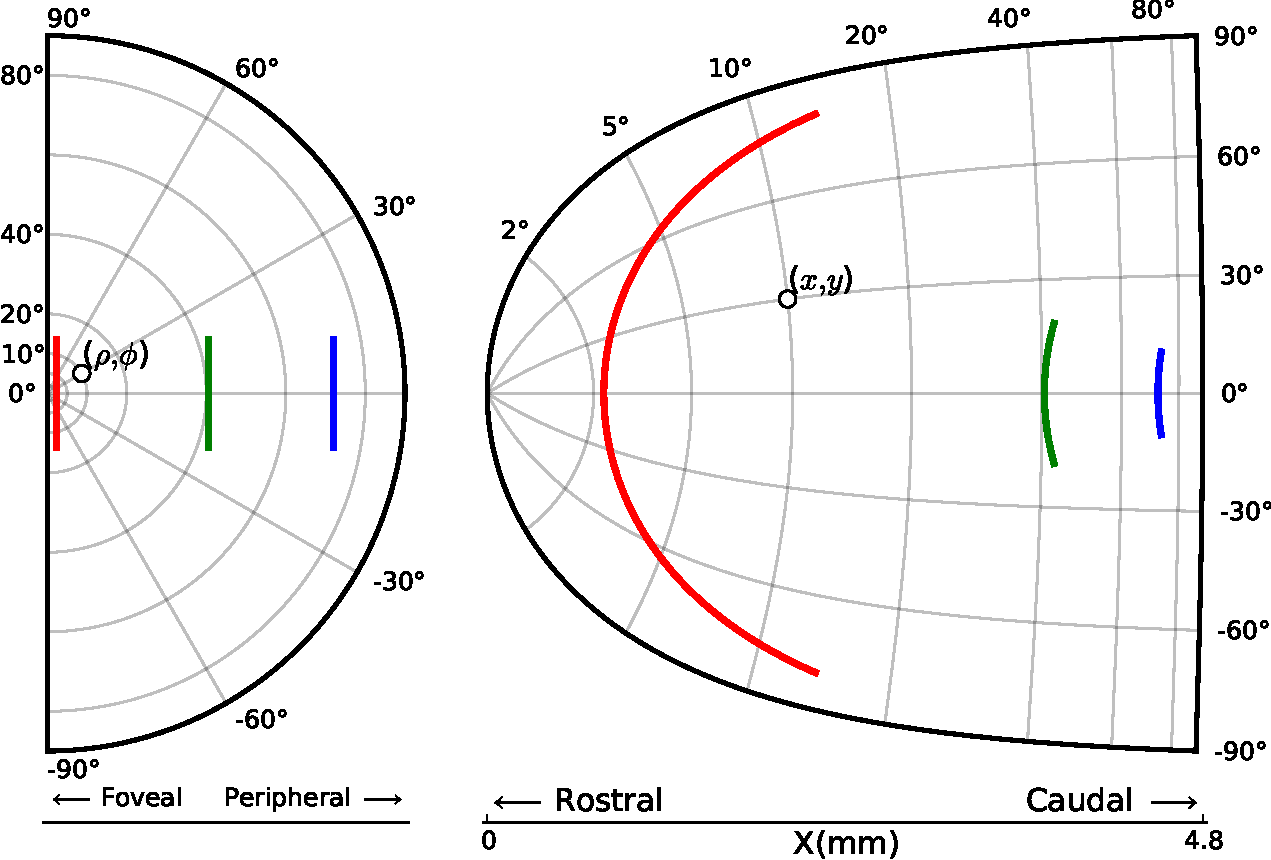
\includegraphics[width=.5\textwidth]{figures/ch3_4_mapping} & 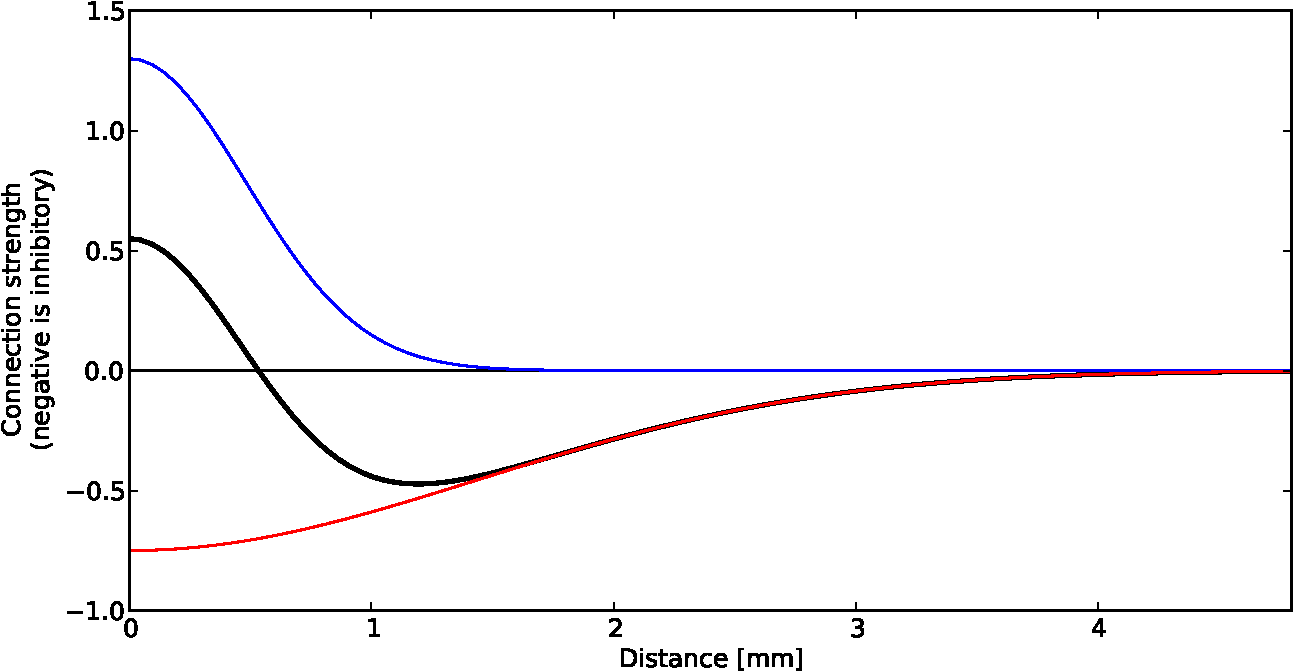
\includegraphics[width=.5\textwidth,height=5cm]{figures/ch3_4_weights-profile}\\
\hline
C&D\\

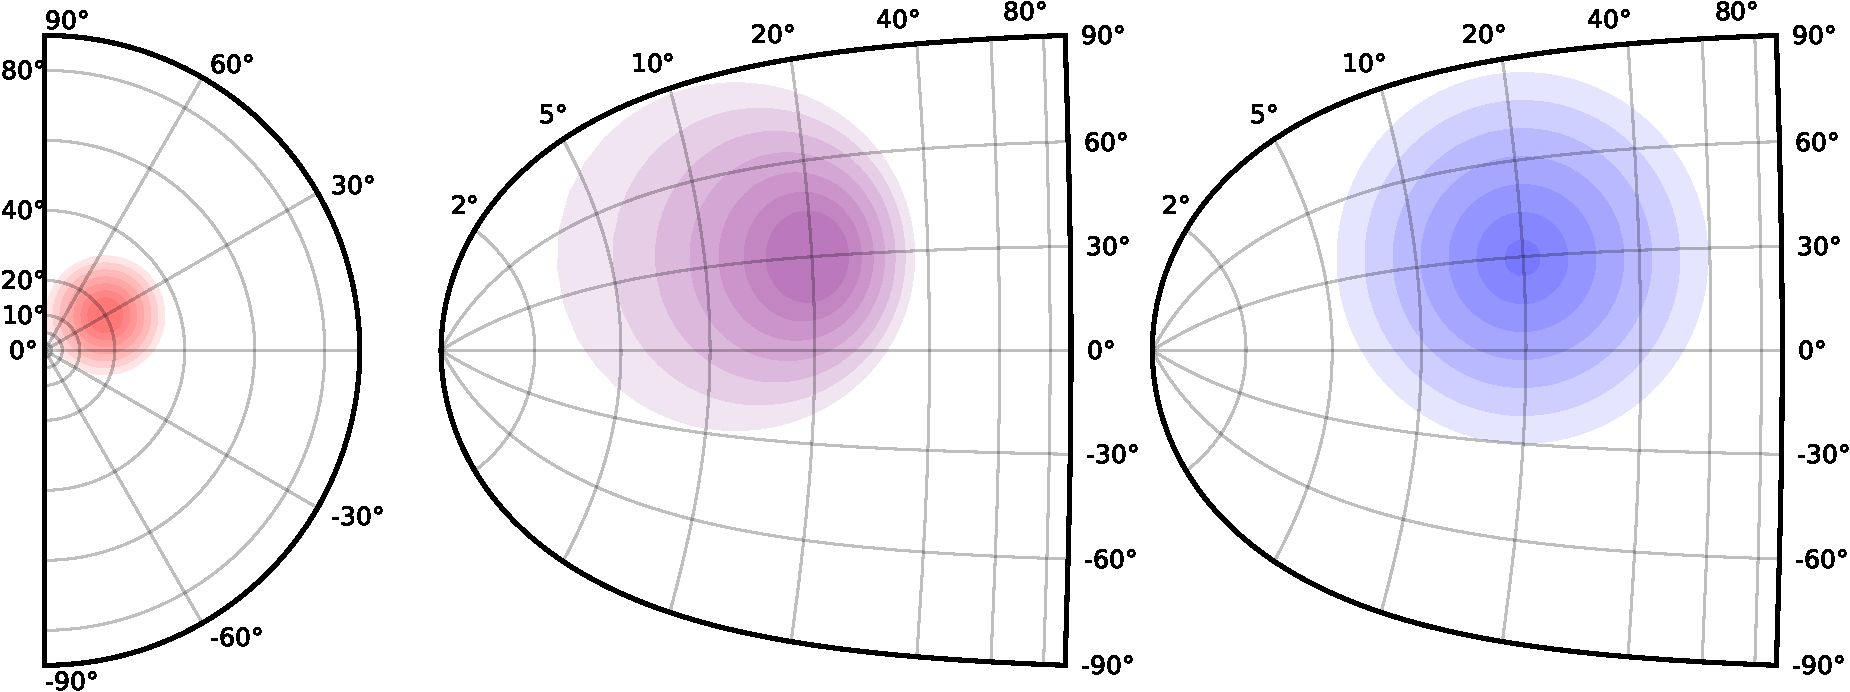
\includegraphics[width=.5\textwidth]{figures/ch3_4_topology}& 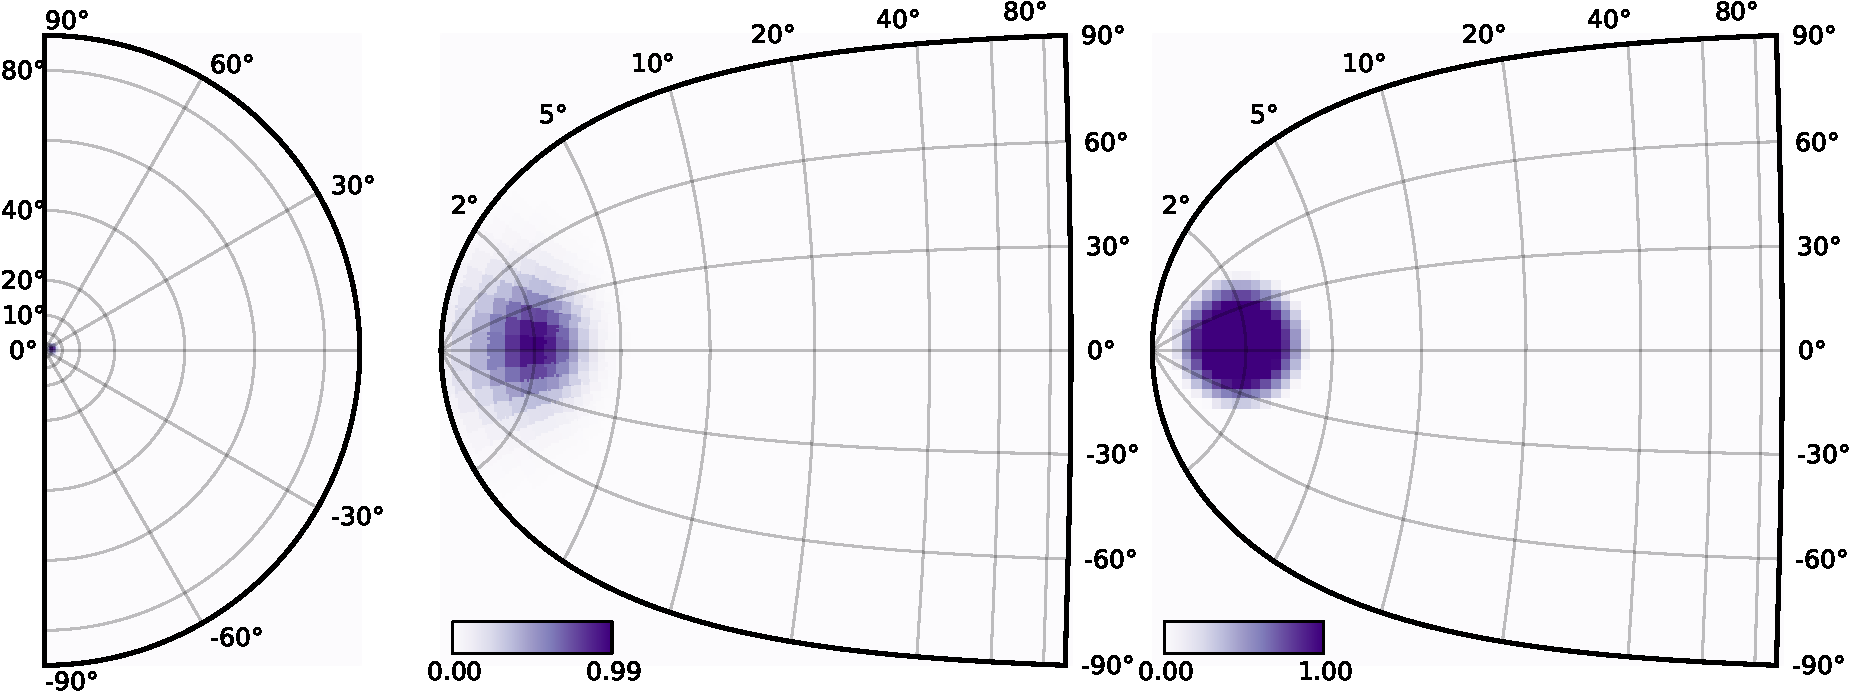
\includegraphics[width=.5\textwidth]{figures/ch3_4_stimulus-1}\\
\hline
\end{tabular}
  \caption{
Description du modèle. A. Projection des coordonnées polaires dans l'espace visuel en coordonnées cartésiennes dans le \protect\gls{sc}. La projection rétinotopique modifie les propriétés géométriques de l'image tout en gardant les relations de voisinage. \protect\`A gauche, l'hémichamp visuel droit (lignes des iso-directions et des demi-cercles d'excentricité constante). \protect\`A droite la carte représentant le colliculus avec des lignes d'iso-amplitudes du \protect\gls{sc} $(2° à 90°)$ et des lignes d'iso-directions $(- 90° à 90°)$ sont indiquées. Les coordonnées polaires visuelles $(\protect\rho, \protect\phi)$ sont transformées en coordonnées colliculaires cartésiennes $(x, y)$ en utilisant les équations \protect\ref{eq: mapping}. Les lignes colorées illustrent la magnification de la représentation des stimuli dans la région fovéale. B. Le pattern des connexions intracolliculaires (noires) résultant de la différence entre une fonction excitatrice locale (bleue) et une fonction inhibitrice globale (rouge). C. Relation topologique entre la surface rétinienne isotropique (rouge), les projections colliculaires anisotropiques correspondant à la présentation d'un stimulus dans le champ visuel (pourpre) et la connectivité latérale isotropique (bleue) dans le colliculus supérieur. D. La projection d'un stimulus visuel gaussien (situé à (2°,0°)). Au milieu, la projection d'entrée à la carte colliculaire. \protect\`A droite l'activité du colliculus supérieur enregistrée après stabilisation de son activité.
}
  \label{fig: mapping}
\end{figure}

En ce qui concerne les détails de la simulation, nous n'avons pas utilisé une fonction explicite du système inverse des équations \ref{eq: mapping} permettant de faire la projection des coordonnées rétiniennes en coordonnées colliculaire. Nous avons plutôt calculé une approximation numérique de la transformation inverse.

\subsection{La carte computationnelle du colliculus}

La couche profonde du \gls{sc} a été modélisée en utilisant la théorie des champs neuronaux dynamiques \cite{Amari:1977, Taylor:1999} décrite dans le premier chapitre selon laquelle un volume cortical donné Ω est considéré comme étant un continuum spatial. Bien que cette théorie ait été proposée pour simuler principalement des activités dans le cortex cérébral, nous avons supposé que la densité neurale dans le \gls{sc} est assez élevée pour nous permettre de transposer cette théorie, comme supposé dans plusieurs autres modèles \cite{Trappenberg:2001, Schneider:2002, Marino:2012}. Le formalisme des \glspl{dnf} propose que la population des unités neurales actives peut être décrite comme un champ continu d'activités. Les unités neurales, comme éléments de la carte, peuvent être considérées comme un ensemble de processeurs homogènes fonctionnant en parallèle sur les signaux entrants. La dynamique du champ est régie par une équation du type :

\begin{align*}
	\frac{1}{\tau} \frac{\partial u({ \vec{z}},t)}{\partial t}
	 = - u({\bf \vec{z}},t)
 	 + \int_{\Omega}^{} w({ \vec{z}},{\vec{z'}})f(u({ \vec{z'}}, t - \frac{|{ \vec{z}-\vec{z'}}|}{v}))d{\vec{z'}}
     + i({\vec{z}},t) 
\end{align*}


o\`u  $u(\vec{z}, t)$ représente l'activité (le potentiel moyen de membrane) à la position $\vec{z}$ à l'instant $t$, $I(\vec{z},t)$ représente l'entrée synaptique reçue à l'instant $t$ et à la position $\vec{z}$, $W$ est une fonction de poids décrivant la force de la connexion entre une unité neurale à la position $\vec{z}$ et une unité à la position $\vec{z'}$, $f$ est la fonction de fréquence de décharge d'une unité neurale simple, $v$ est la vitesse de conduction d'un potentiel d'action et $\tau$ est une constante de temps caractéristique de l'activation des neurones. \'Etant donnée la petite taille du colliculus , la vitesse de conduction a été négligée $(v=+\infty)$ et le champ de l'activité colliculaire a été considéré comme homogène et isotrope, ce qui mène à l'équation simplifiée suivante :\\
%1/τ (∂u (⃑ de z, t))/∂t=-u (⃑ de z, t)+∫_SC▒w (|^ de ⃑-z ⃑ de z ' |) f (u (⃑ de z, t)) DZ ⃑'+i (⃑ de z, t)    (5)
\begin{align}
	\frac{1}{\tau} \frac{\partial u({\vec{z}},t)}{\partial t}
	 = - u({ \vec{z}},t)
 	 + \int_{\Omega}^{} w(|{\vec{z}}-{\vec{z'}}|)f(u({\vec{z'}}, t))d{ \vec{z'}}
     + i({\vec{z}},t)
  \label{eq: neural_field}
\end{align}

Pour la fonction f de fréquence de décharge, nous avons employé une fonction simple $f(u)=min(max(u, 0), 1)$ \footnote{le 1 correspond à la fréquence de décharge maximale (qui sera considérée égale à 500Hz dans la simulation) } puisque c'est la fonction la plus simple qui peut fournir la stabilité pour un tel champ \cite{Salinas:1996}.\\

La densité des unités neurales dans le \gls{sc} est considérée constante le long de la surface colliculaire et nous considérons que la force des connexions latérales excitatrices et inhibitrices est représentée par une fonction qui dépend de la distance entre les cellules mesurées sur la surface du \gls{sc} i.e. [$ w(\vec{z},\vec{z'})=w(\vert \vec{z}-\vec{z'} \vert)$]. La connectivité latérale d'une cellule donnée est ainsi isotrope (fig \ref{fig: mapping}-C), contrairement à \cite{Nakahara:2006} où les connexions sont basées sur la proximité des stimuli. Considérons deux cellules à deux positions respectives $\vec{z}$ et $\vec{z'}$, la force de connexions résultante est définie par:\\

\begin{align}
w(\vec{z},\vec{z'})=E~exp\left(-\frac{\vert \vec{z}-\vec{z'} \vert^2}{{\sigma_e}^2}\right) -
  I~exp\left(-\frac{\vert \vec{z}-\vec{z'} \vert^2}{{\sigma_i}^2}\right)
  \label{eq: weight}
\end{align}

o\`u $E$, $I$ sont les amplitudes, $\sigma_e$, $\sigma_i$, sont respectivement les écarts types des fonctions gaussiennes excitatrices et inhibitrices. Nous avons considéré pour nos simulations $\sigma_i \gg \sigma_e$, ce qui correspond à des connexions inhibitrices à longue portée (globales) et des connexions excitatrices à courte portée (locales).\\

Les effets de l'inactivation locale dans le \gls{sc} ont été simulés numériquement en multipliant la matrice d'activation $U$ résultant de l'équation (eq \ref{eq: neural_field}) par une matrice binaire $L$ (un masque) dans laquelle un état d'activation est attribué à chaque unité ($1$ pour une unité d'active et $0$ pour inactivée). Dans les expériences, le modèle de lésion que nous employons est une matrice avec un disque uniforme de valeurs nulles.\\

\subsection{Le d\'ecodage de l'activité colliculaire}

Comme passé en revue dans \cite{Gandhi:2011}, plusieurs schémas de décodage de l'activité du \gls{sc} ont été proposés.  Sauf indication contraire, le déplacement désiré de l'oeil $\vec{\Delta E}$  est décodé en utilisant un vecteur de moyenne statique:

\begin{align}
  \Delta\vec{E} = \frac{\sum_{\substack{\Omega}}^{} r_z\vec{R}_z }{\sum_{\Omega}^{}r_z}
\label{sommation}
\end{align}

avec $r_z$ est la fréquence moyenne de décharge d'une cellule à une position donnée $\vec{z}$ et $\vec{R}_z$  est le vecteur de déplacement préféré codé par cette cellule. Nous n'avons pas choisi le schéma de décodage par somme car l'activation obtenue n'est pas parfaitement stéréotypée, le nombre d'unités actives en réponse à un stimulus est constant mais l'activation maximale varie selon l'excentricité. \\


\section{Résultats}

\subsection{\' Etendue de la population active}

Nous avons examiné l'étendue de la population active dans la carte du \gls{sc} qui résulte de la présentation de stimuli identiques à différents emplacements du champ visuel. L'entrée de la carte colliculaire est différente pour chaque stimulus en raison de la déformation logarithmique (fig \ref{fig: mapping}-C et \ref{fig: mapping}-D). En effet, à cause de la projection non linéaire de la carte rétinienne sur la carte du \gls{sc}, un stimulus apparaissant dans le champ visuel central\footnote{On distinguera dans les descriptions des positions des stimuli, les stimuli centraux correspondant à des projections fovéales sur la rétine et rostrales sur le colliculus et les stimuli périphériques correspondant à des projections périphériques sur la rétine et caudales sur le colliculus} active initialement une population d'unités neurales colliculaires plus grande que celle activée par des stimuli plus périphériques. Cependant, après plusieurs pas de calcul, la distribution de l'activité colliculaire atteint un état stable ayant toujours la même forme et la même étendue spatiale de la population active, sans se soucier de l'excentricité de la cible dans le champ visuel. On parle donc d'une bulle d'activité ``stéréotypée'' (en étendue et non pas en amplitude à cause la décroissance de l'activation maximale des neurones avec l'excentricité comme montré dans la suite). Cet état final résulte du profil imposé à la connectivité latérale. La distribution de l'activité sur la carte se rapproche d'une gaussienne (2D) quand elle se stabilise. L'étendue de la connectivité excitatrice détermine la taille finale de la population active (puisque l'inhibition est supposée être globale). 

\subsection{Champs récepteurs}

Nous avons de même examiné la réponse des unités neuronales situées à différents emplacements dans la carte du \gls{sc} en réponse à des stimuli présentés à différentes excentricités dans la carte de la rétine. \\

\begin{figure}[ht]
  \begin{center}
    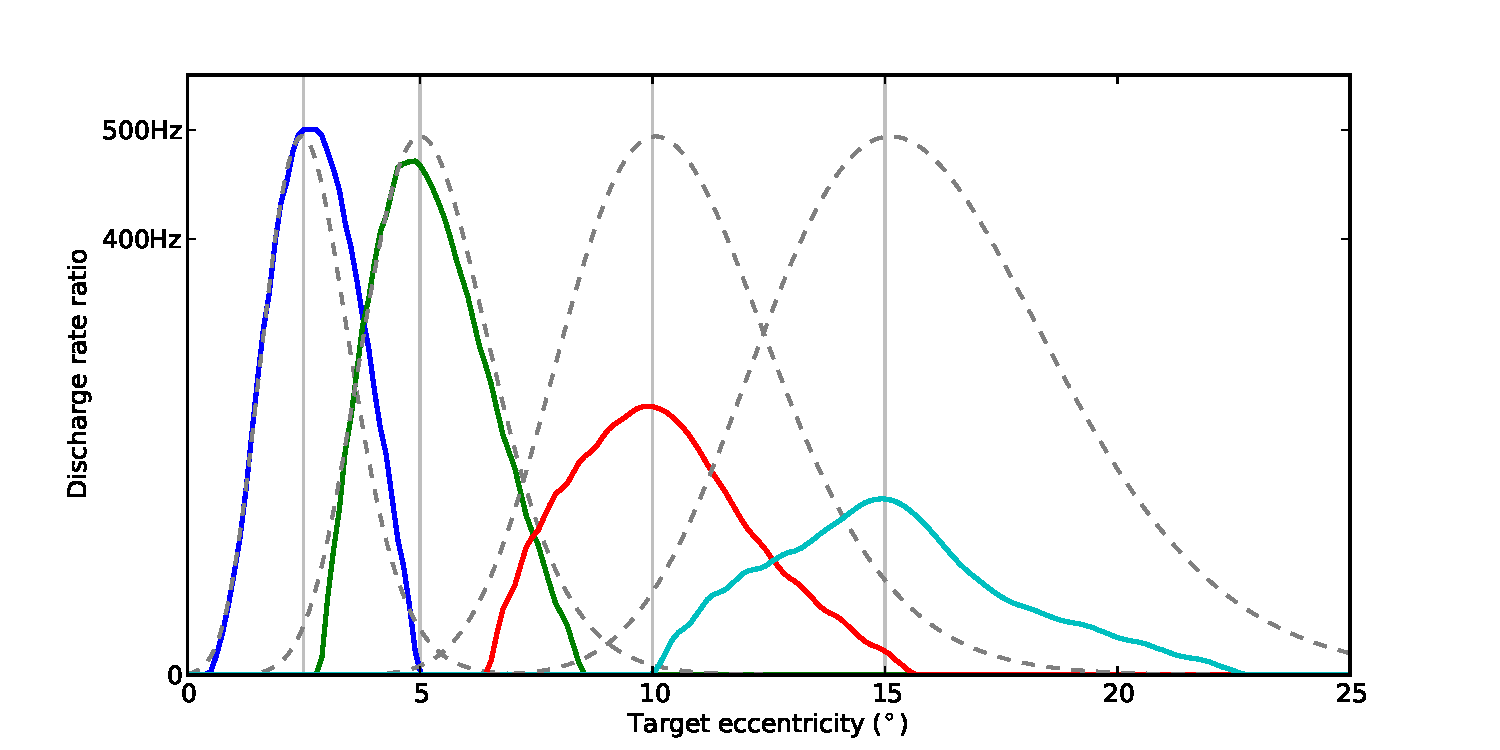
\includegraphics[width=0.8\textwidth]{figures/ch3_5_RF}
  \end{center}
  \caption{ Champs récepteurs. Réponse neuronale (4 neurones) à un stimuli présenté successivement à des excentricités variant de 1° à 25°. Pour chacun des 4 neurones (situés respectivement à une excentricité d'à peu près 2.5°, 5°, 10° et 15° et une amplitude de 0° pour tous sur la carte colliculaire selon la projection logarithmique). L'activation maximale (fréquence de décharge) est mesurée à la convergence du système. La largeur des champs récepteurs décroît avec l'excentricité. Les pointillés représentent les entrées (l'activation initiale).}
  \label{fig: receptive-field}
\end{figure}

La figure (fig \ref{fig: receptive-field}) montre que le champ récepteur\footnote{Le champ récepteur d'une cellule neuronale colliculaire est l'intervalle des excentricités des cibles pour lesquelles cette unité s'active} d'une unité dépend de l'emplacement de cette unité dans la carte colliculaire. La réponse est maximale pour une excentricité préférée, diminue en s'éloignant de part et d'autre de cette excentricité (c'est à dire diminue pour des excentricités plus petites ou plus grandes) et disparaît pour des saccades vers des emplacements qui sont relativement très loin de l'excentricité préférée. La forme des champs est un peu asymétrique et plus l'emplacement préféré est excentré, plus la courbe d'accord est large.

\subsection{Exactitude}

En utilisant le décodage par moyenne (eq \ref{sommation}), nous avons examiné l'exactitude (\textit{accuracy}) du modèle en présentant des cibles à divers emplacements dans le champ visuel. La figure (fig \ref{fig: accuracy}-A) montre, le long de la carte colliculaire, les emplacements théoriques des stimuli par des petits cercles pleins et les emplacements résultant du décodage par des petits cercles vides. Malgré la transformation log-polaire de la carte rétinienne et le codage distribué des localisations des cibles (plusieurs unités s'activent pour une cible donnée), l'exactitude du modèle est assez satisfaisante, la distance angulaire moyenne entre les emplacements théoriques et les emplacements décodés après une seconde de com vaut $3.10^{-3}$. Quand des stimuli ont été présentés dans la zone fovéale, le biais du décodage (le décalage entre les cercles vides et pleins) de la cible sur le \gls{sc} est dans le sens de la partie périphérique du champ visuel et inversement le biais est plus dirigé vers la partie centrale quand les mêmes stimuli sont présentés dans la zone périphérique. Les biais de position sont plus fréquents sur les bords du \gls{sc}, i.e. dans les régions colliculaires codant des cibles sur la fovéa ou sur le méridien vertical.


\begin{figure}
  \begin{center}
    \begin{tabular}[t]{cc}
     {\textsf {\textbf A}} &
      {\textsf {\textbf B}} \\
      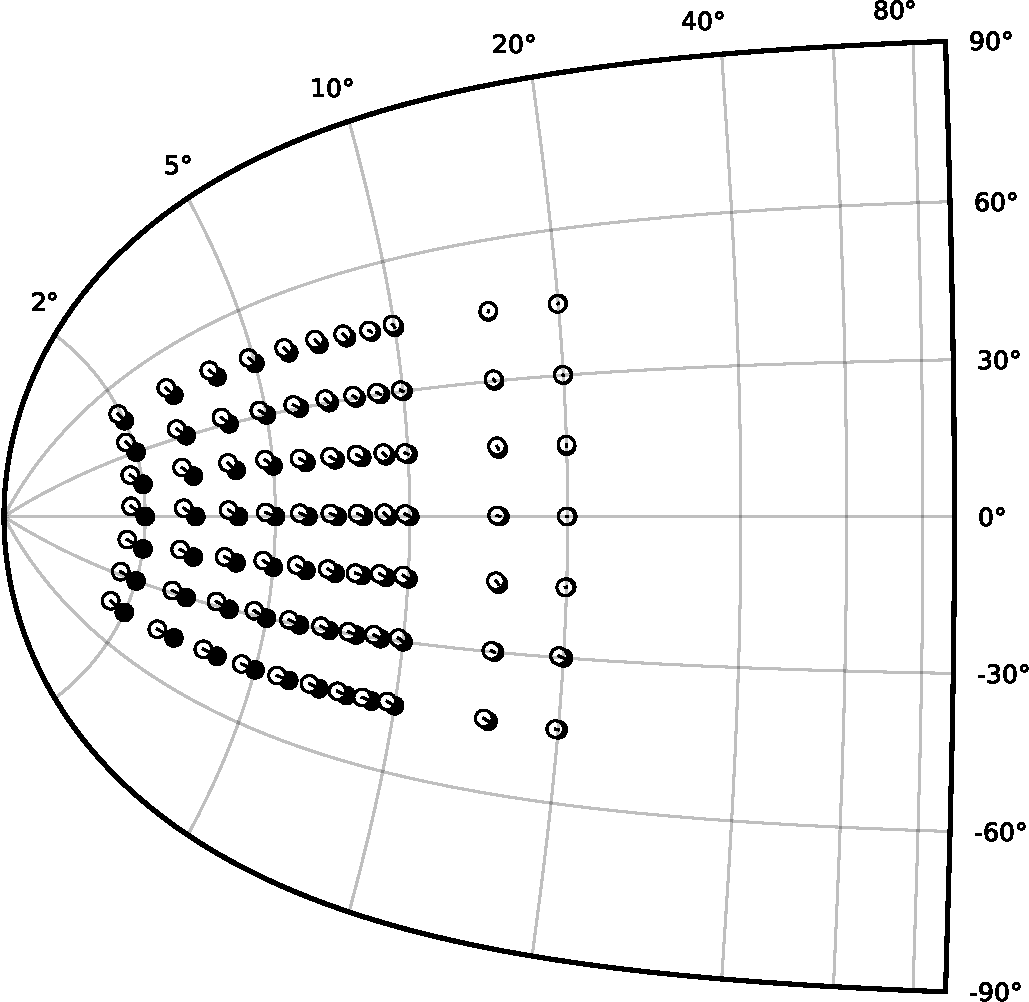
\includegraphics[width=0.4\textwidth]{figures/ch3_6_lesion-1} &
      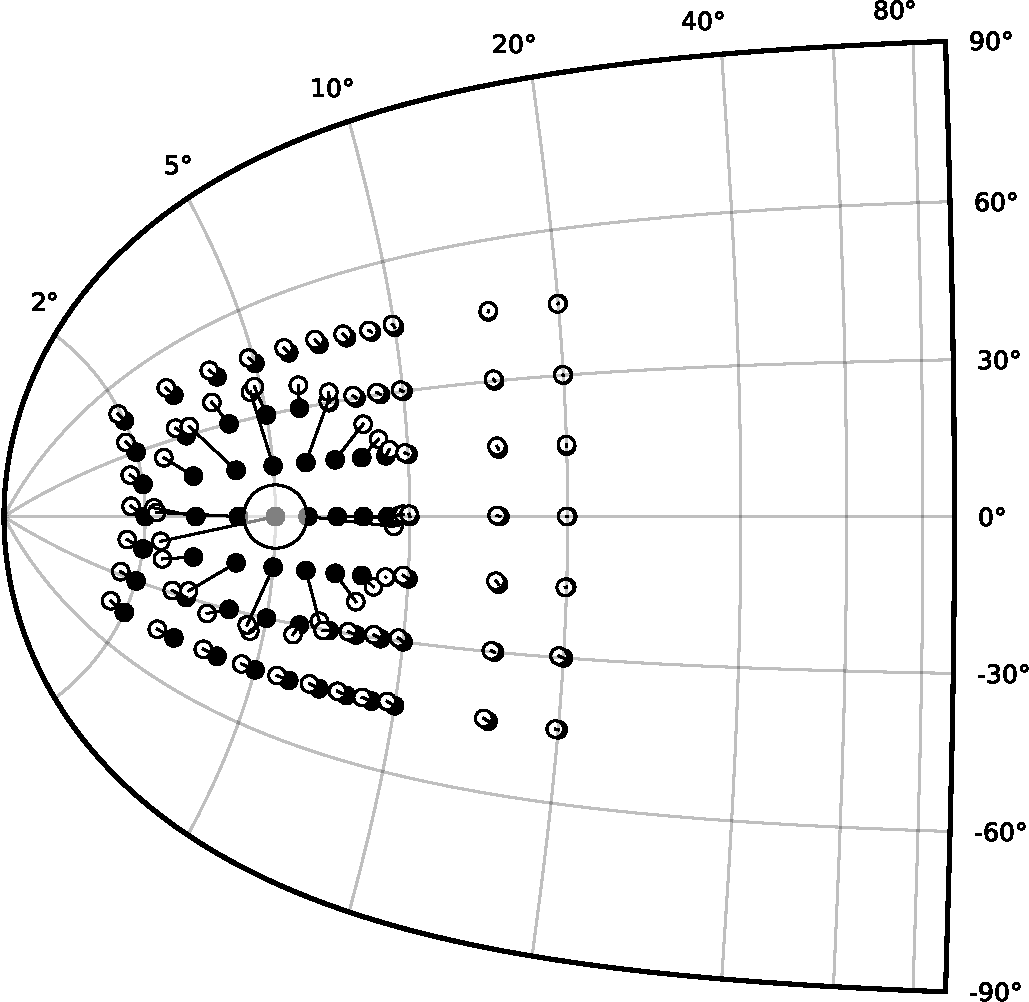
\includegraphics[width=0.4\textwidth]{figures/ch3_6_lesion-2} \\
      {\textsf {\textbf C}} &
      {\textsf {\textbf D}} \\     
      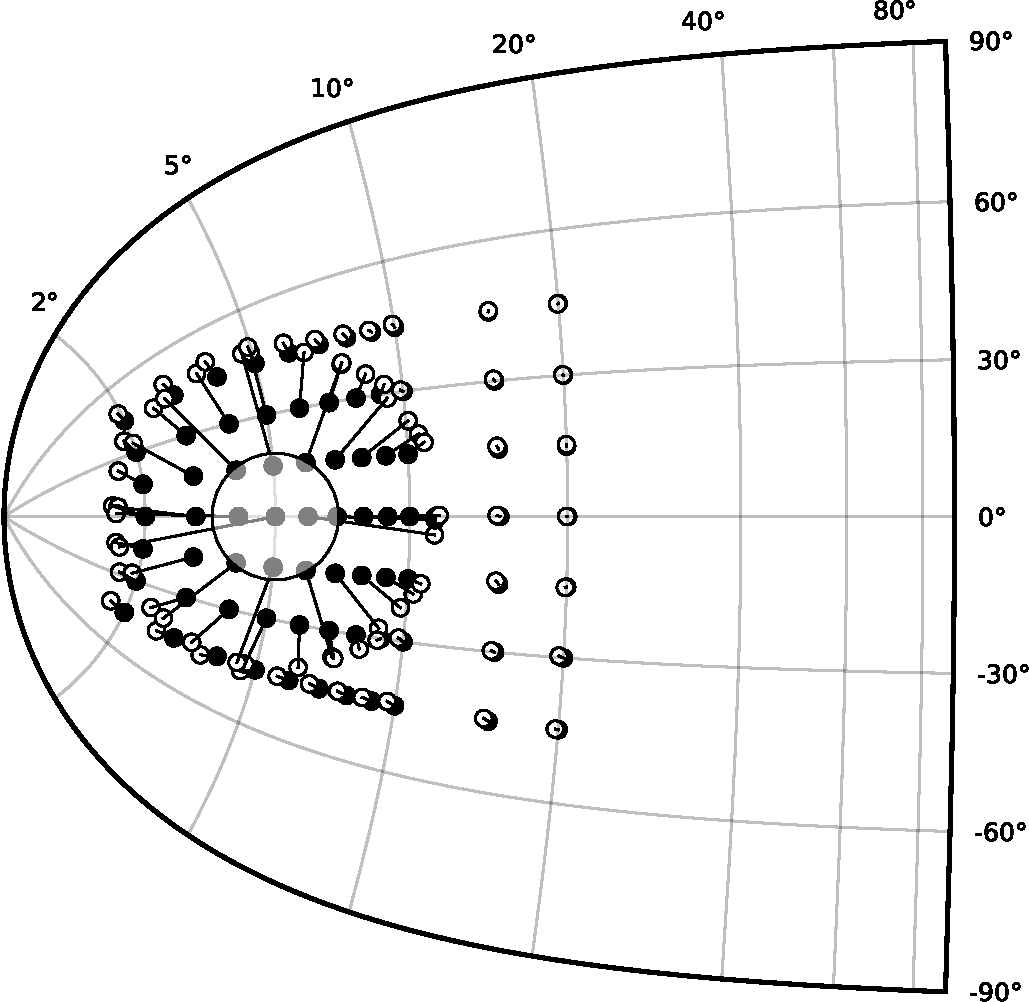
\includegraphics[width=0.4\textwidth]{figures/ch3_6_lesion-3} &
      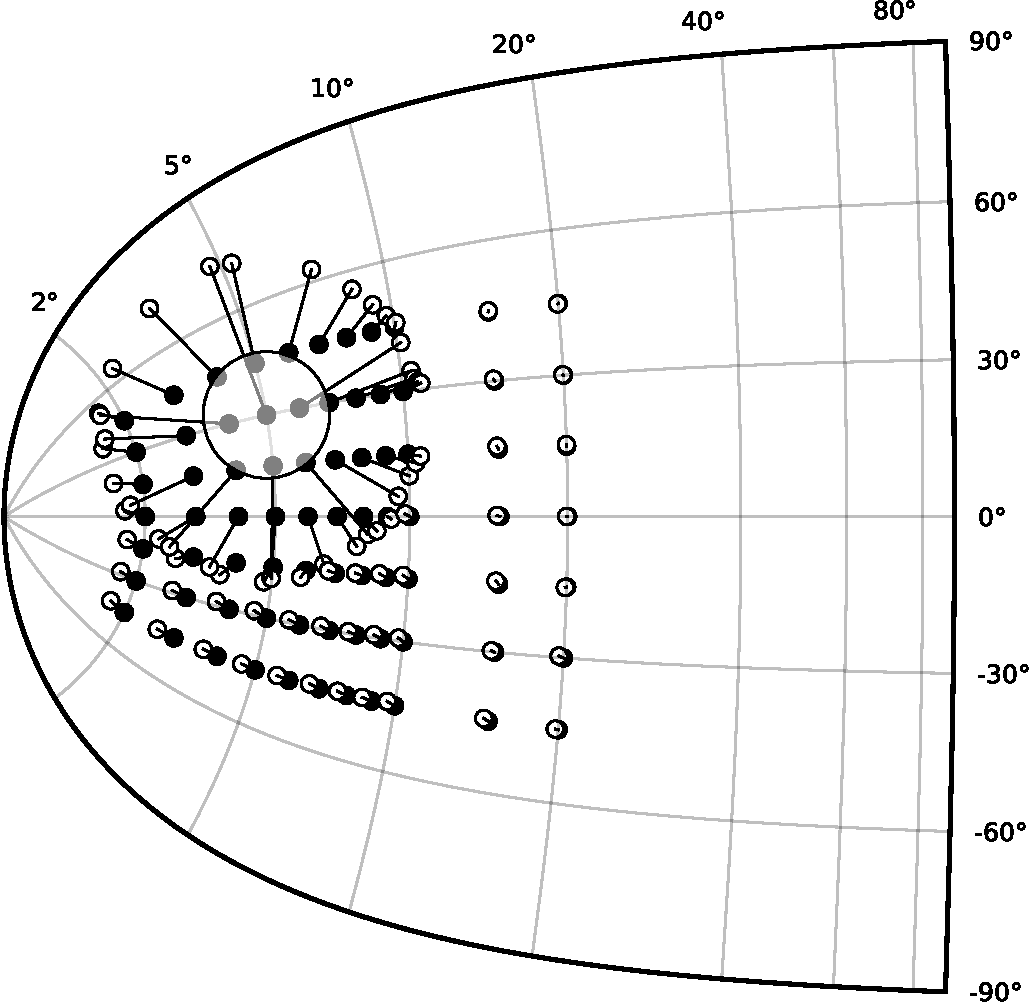
\includegraphics[width=0.4\textwidth]{figures/ch3_6_lesion-4} \\
    \end{tabular}
    \begin{tabular}[t]{cccc}  
      {\textsf {\textbf E}} &
      {\textsf {\textbf F}} &
      {\textsf {\textbf G}} &
      {\textsf {\textbf H}} \\
      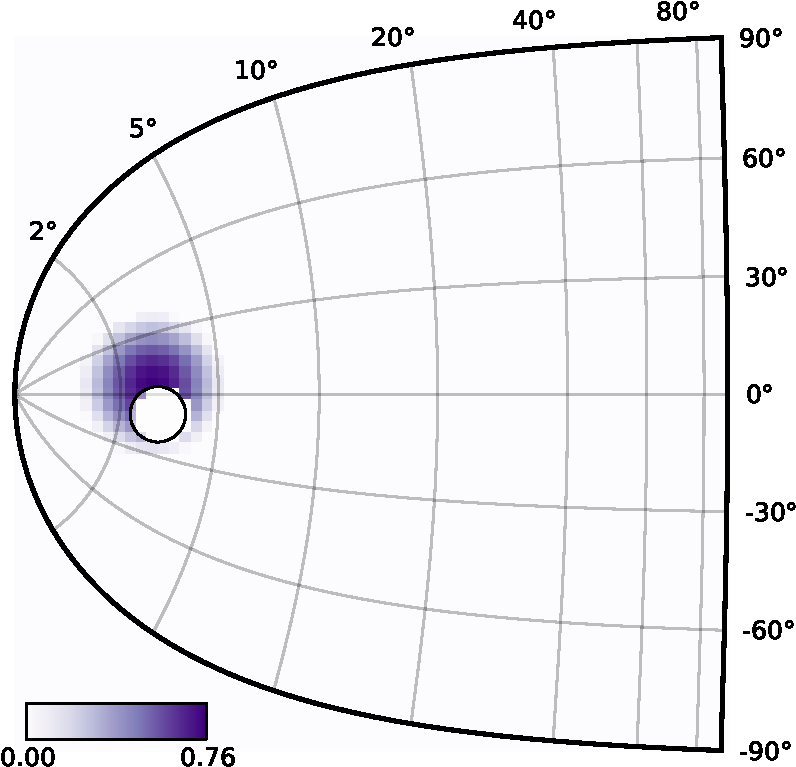
\includegraphics[width=0.23\textwidth]{figures/ch3_6_lesion-after-5} &
      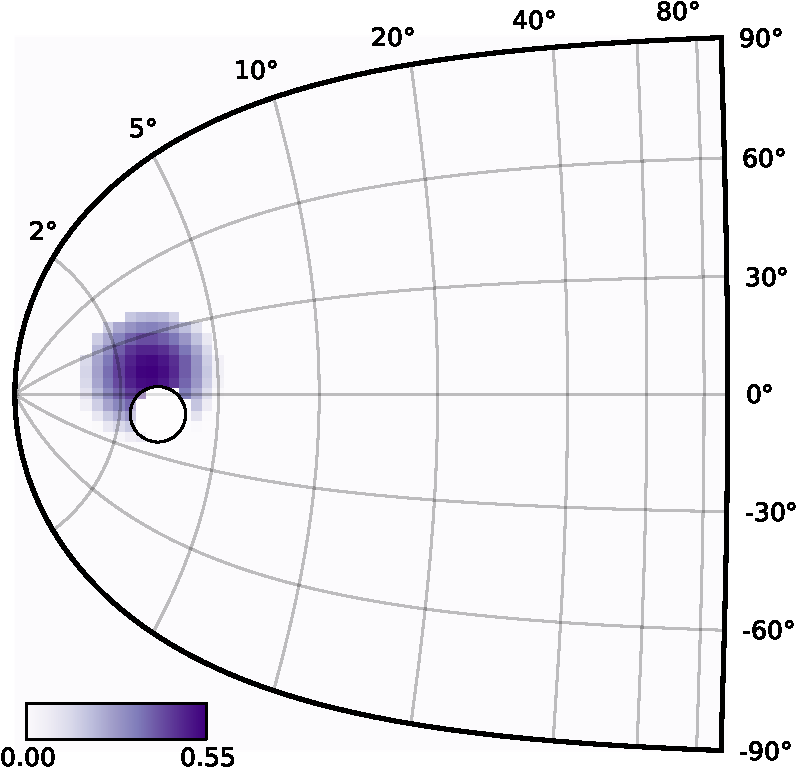
\includegraphics[width=0.23\textwidth]{figures/ch3_6_lesion-after-25} &
      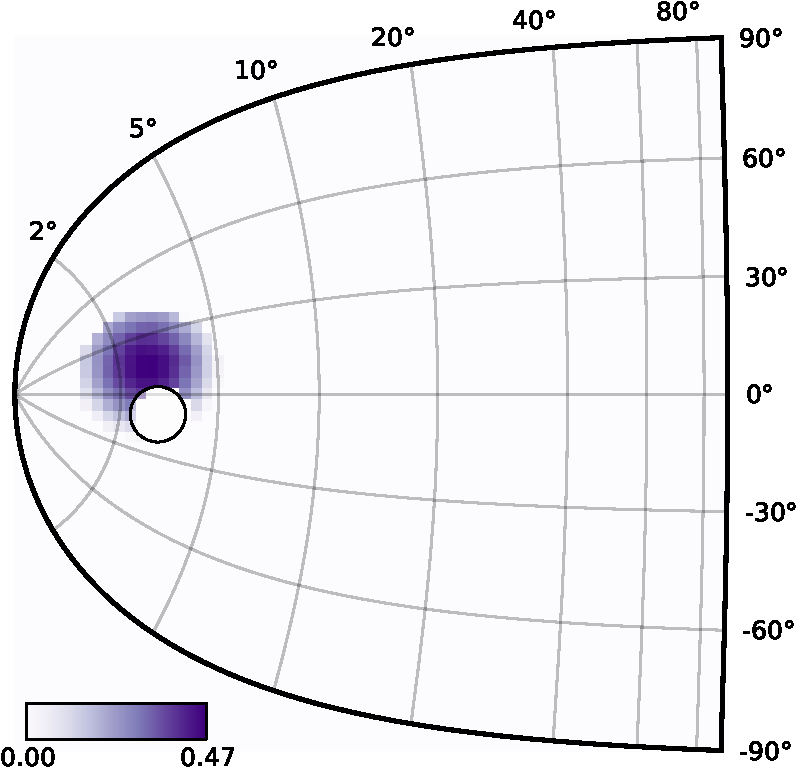
\includegraphics[width=0.23\textwidth]{figures/ch3_6_lesion-after-50} &
      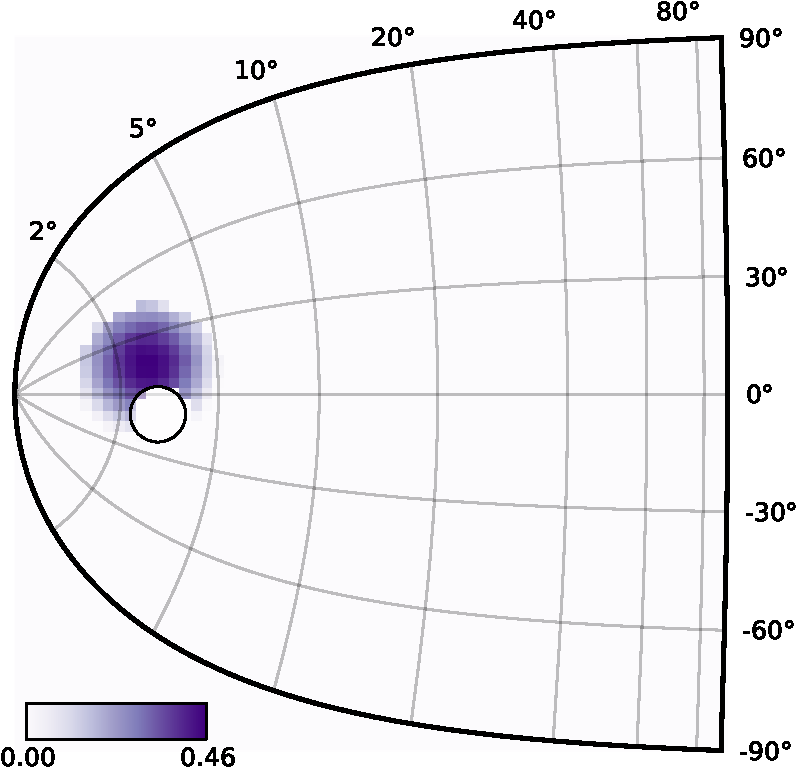
\includegraphics[width=0.23\textwidth]{figures/ch3_6_lesion-after-100}  \\
    \end{tabular}
  \end{center}

  \caption{Exactitude du décodage et effet des lésions sur l'activité colliculaire. L'exactitude du modèle a été examinée sur un ensemble de cibles à des emplacements différents présentés séquentiellement au modèle. Pour chaque cible, le centre de masse de l'activité colliculaire est décodé et représenté par un cercle (vide) alors que la position théorique est représentée par un cercle plein. A. Le modèle sans lésions. B. Une petite lésion circulaire à la position (5°, 0°). C. Une lésion de taille moyenne à la position (5°, 0°). D. Une lésion de taille moyenne à la position (5°, 30°). E.F.G.H. Effet de l'inactivation sur l'activation de la carte colliculaire à différents pas (respectivement 5ms, 25ms, 50ms et 100ms après l'apparition du stimulus). La population active se décale loin du site de la lésion. }
  \label{fig: accuracy}
\end{figure}


\subsection{Temps de r\'eponse}

Nous avons étudié l'effet de la taille, l'intensité et l'excentricité du stimulus rétinien sur la réponse colliculaire. La figure (fig \ref{fig: time}) montre l'évolution temporelle de l'activation maximale (fréquence de décharge) en fonction du temps pour plusieurs excentricités en fixant la taille et l'intensité aux valeurs standards (fig \ref{fig: time}-A), pour plusieurs tailles du stimulus en fixant l'excentricité à 5 et l'intensité à 1 (fig \ref{fig: time}-E) et pour plusieurs intensités en fixant la taille à 1 et l'excentricité à 5 (fig \ref{fig: time}-C).\\

Le temps de latence d'une saccade est défini comme le temps écoulé entre la présentation d'une cible et le déclenchement des saccades. C'est par rapport à cette notion qu'on définit donc le temps de réponse de notre modèle. Nous avons choisi un seuil arbitraire de fréquence de décharge maximale à partir duquel on suppose qu'une saccade peut être déclenchée (400HZ).  Mais si on revient aux courbes d'accord, les neurones les plus excentrés ne sont pas capables d'atteindre des seuils d'activation élevés, donc le seuil qu'on avait défini ne s'applique qu'aux stimuli qui se projettent sur la zone rostrale. Un autre critère pourrait être utilisé, à savoir le temps nécessaire pour que l'activation sur la carte colliculaire atteigne un état plus stable\footnote{On suppose que la bulle d'activité est stabilisée quand la variation de la somme des activités entre t et t+1 devient inférieure à une petite valeur $epsilon$}. En examinant les courbes A,C et E, on peut prédire qu'on va obtenir des effets contradictoires avec ceux obtenus par le critère du seuil (moins l'état final est élévé, moins la croissance de la courbe est rapide et plus le temps de stabilisation est court).\\

Les courbes de variations de temps de réponse en fonction des 3 critères: excentricité, taille et intensité sont tracées respectivement dans les figures (fig \ref{fig: time}-B),(fig \ref{fig: time}-D) et (fig \ref{fig: time}-F). Les points de saturation à 500 ms correspondent aux valeurs de variables qui n'ont pas permis d'atteindre le seuil d'activation (choix numérique). En ce qui concerne l'influence de la taille (fig \ref{fig: time}-E et \ref{fig: time}-F ) et l'intensité du stimulus (fig \ref{fig: time}-C et \ref{fig: time}-D), le temps de réponse décroît avec l'augmentation de ces deux paramètres. En effet, plus l'activation initiale est importante, plus l'augmentation des activités individuelles est rapide (excitations mutuelles). \\

Si on varie l'excentricité, on a l'effet inverse. En effet, moins le stimulus est excentré, plus l'activation initiale est importante à cause de la magnification et par la suite plus l'atteinte du seuil de déclenchement est rapide.\\ 

Nous gardons donc le premier critère, en supposant en plus qu'une correction supplémentaire pourrait s'ajouter à la sortie du colliculus permettant d'amplifier les activations caudales pour donner aux générateurs de motifs moteurs une activation stéréotypée (par exemple, ajouter une fonction qui dépend exponentiellement de la position horizontale dans la carte).






\begin{figure}
  \begin{center}
    \begin{tabular}[t]{cc}
     {\textsf {\textbf A}} &
      {\textsf {\textbf B}} \\
      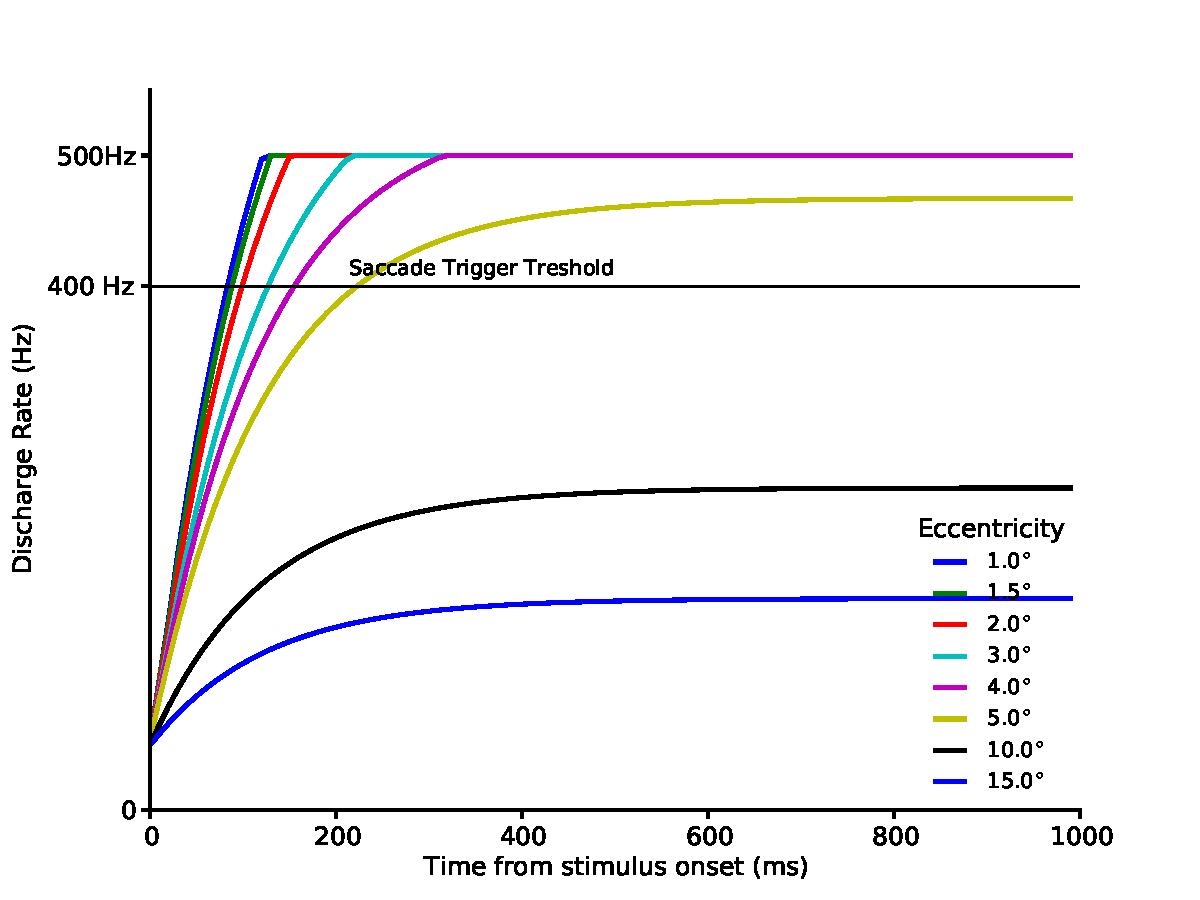
\includegraphics[width=0.5\textwidth]{figures/ch3_7_RT-eccentricity-A} &
      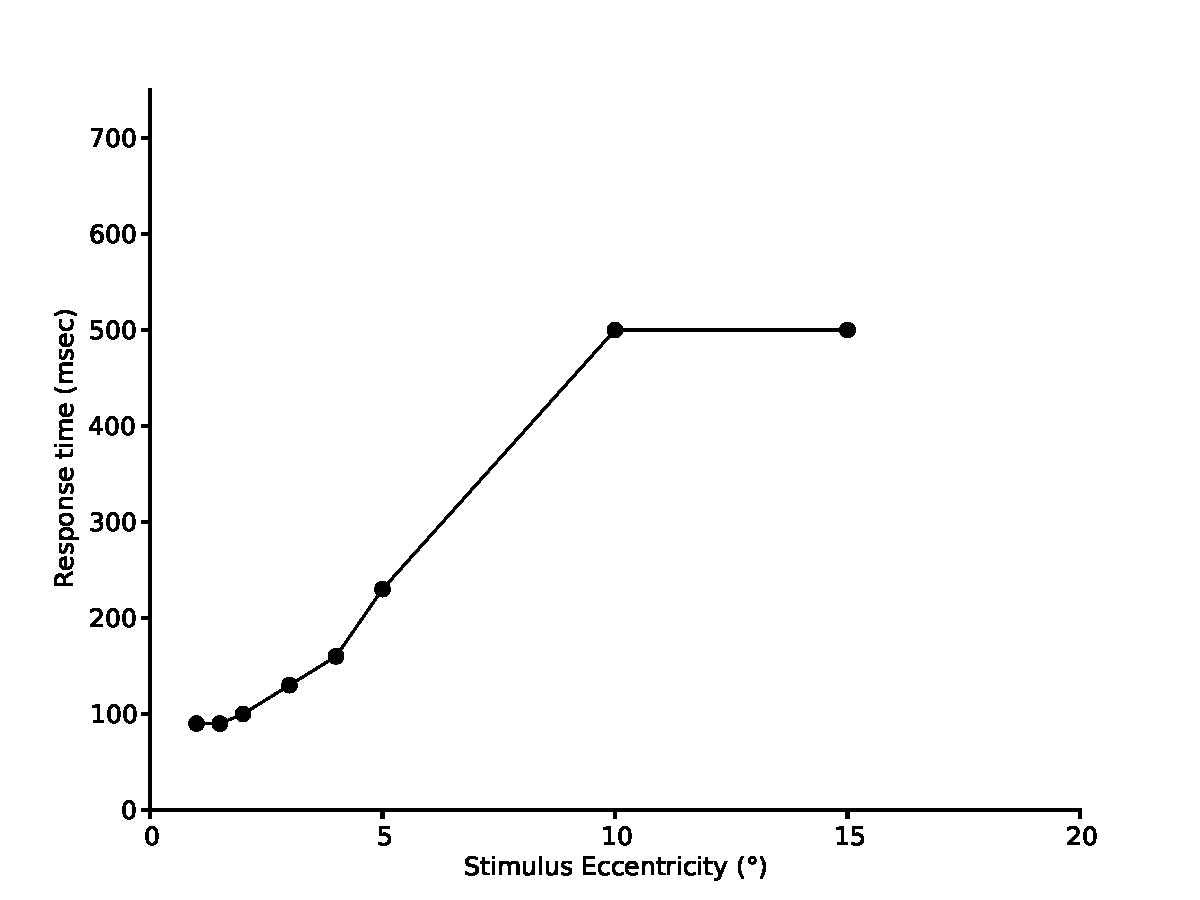
\includegraphics[width=0.5\textwidth]{figures/ch3_7_RT-eccentricity-B} \\
      {\textsf {\textbf C}} &
      {\textsf {\textbf D}} \\     
      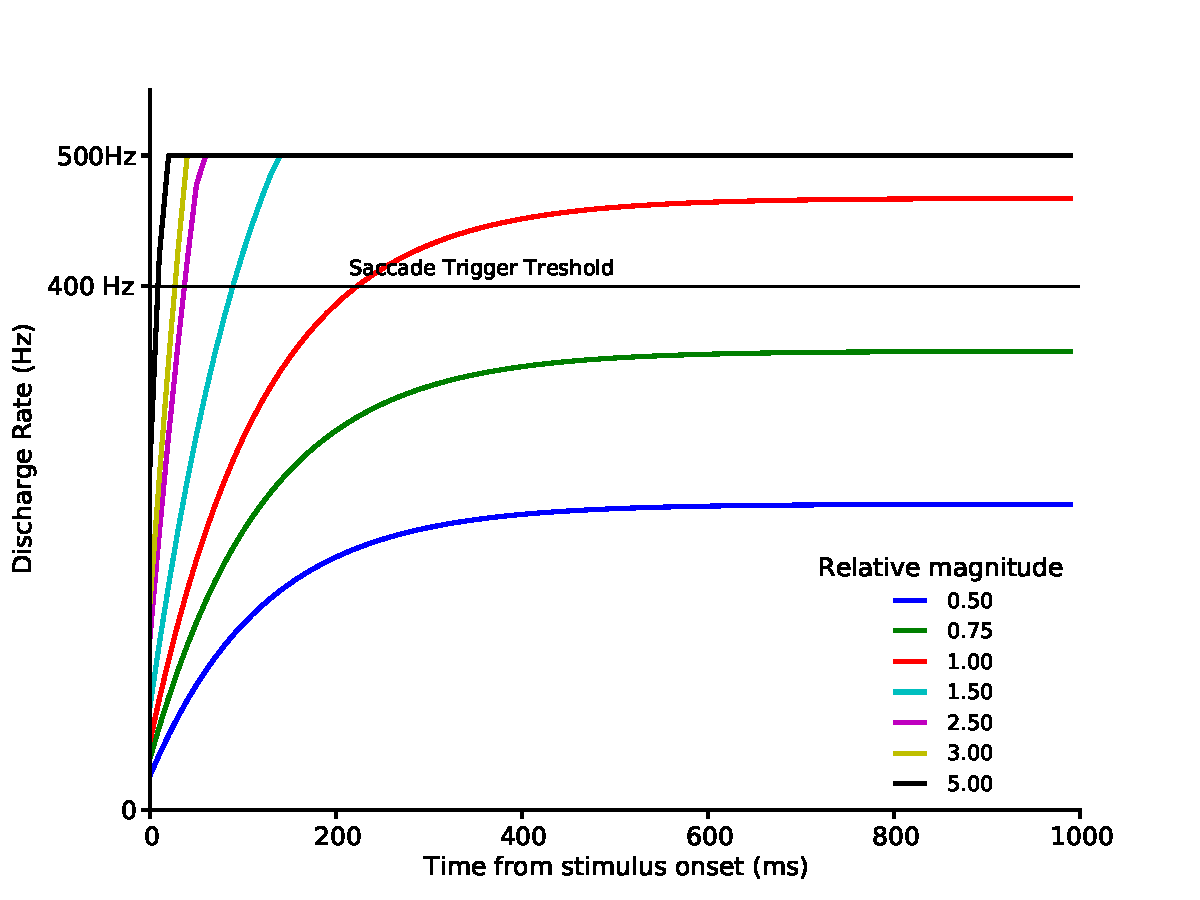
\includegraphics[width=0.5\textwidth]{figures/ch3_7_RT-size-A} &
      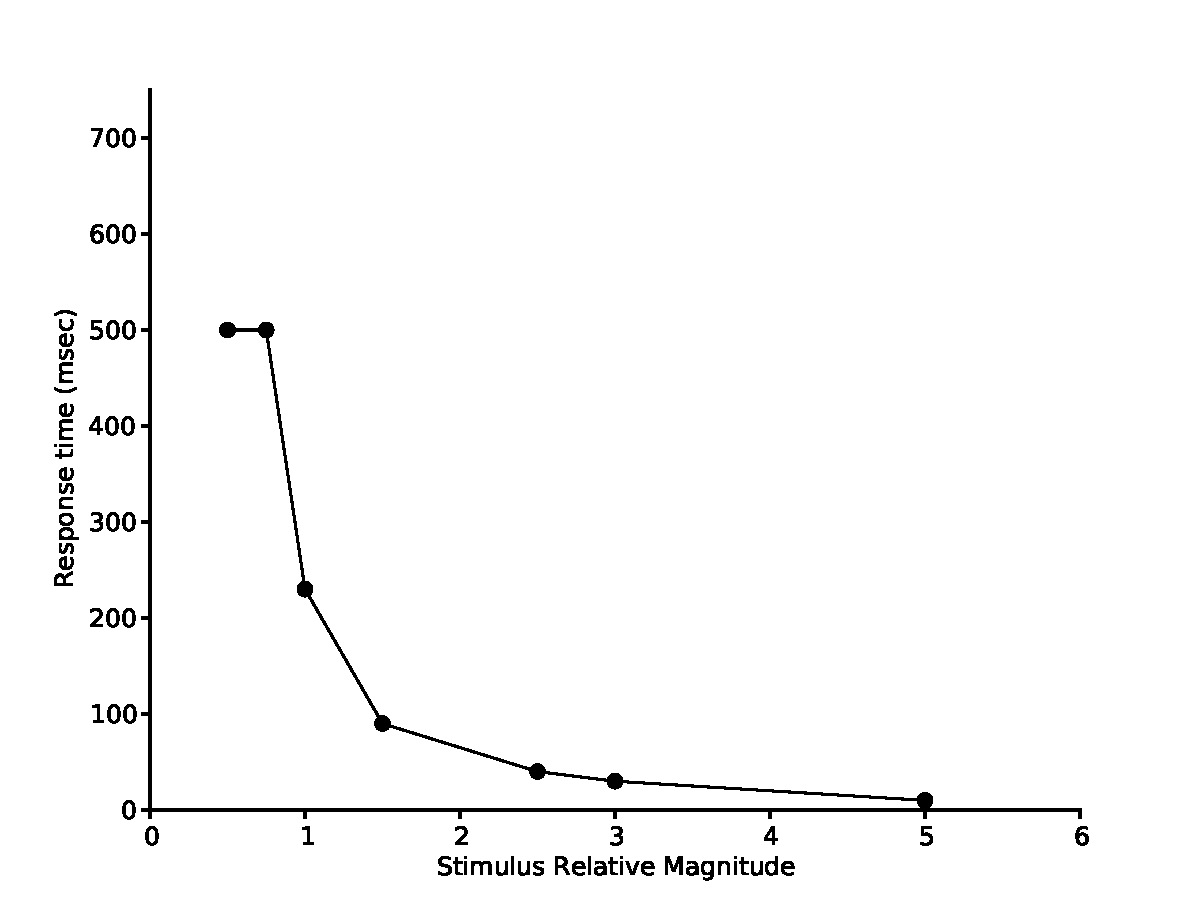
\includegraphics[width=0.5\textwidth]{figures/ch3_7_RT-size-B} \\
      {\textsf {\textbf E}} &
      {\textsf {\textbf F}} \\     
      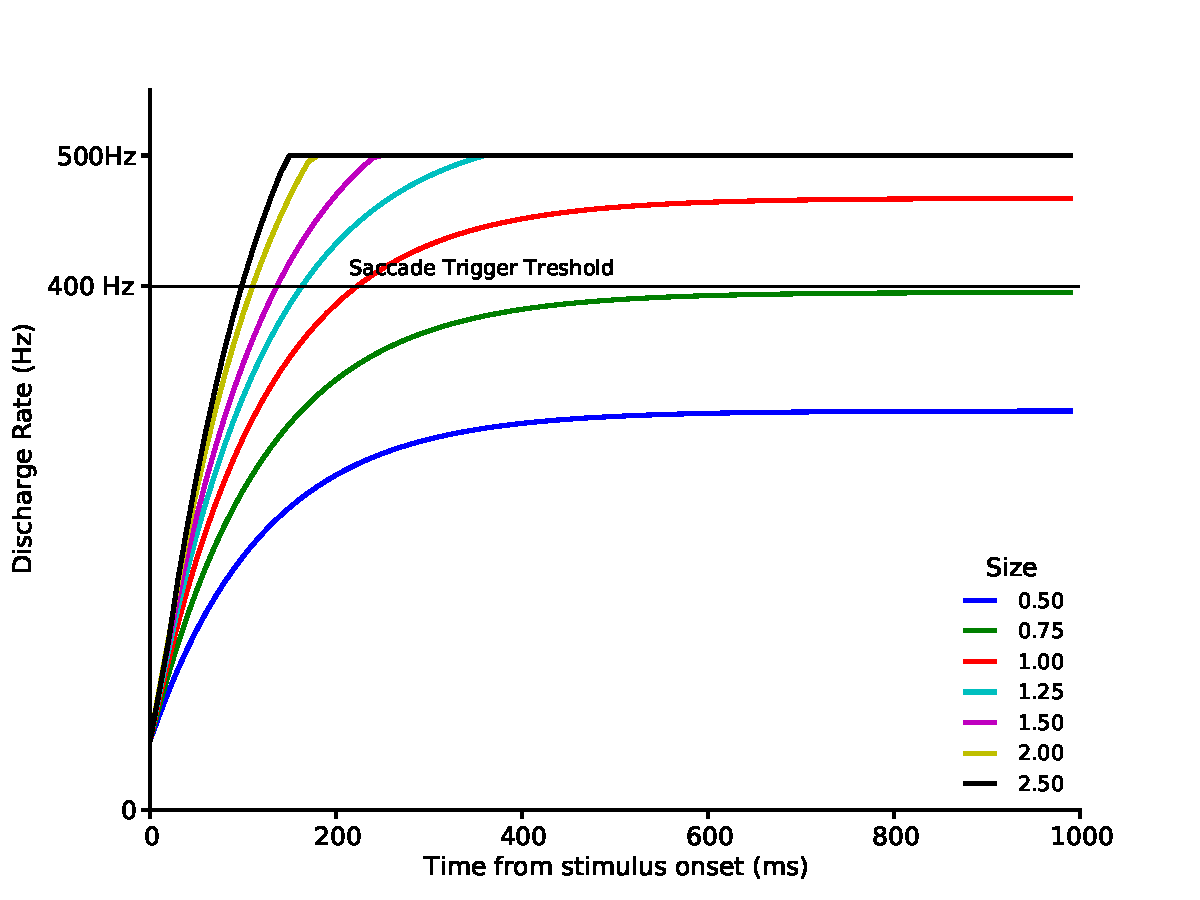
\includegraphics[width=0.5\textwidth]{figures/ch3_7_RT-magnitude-A} &
      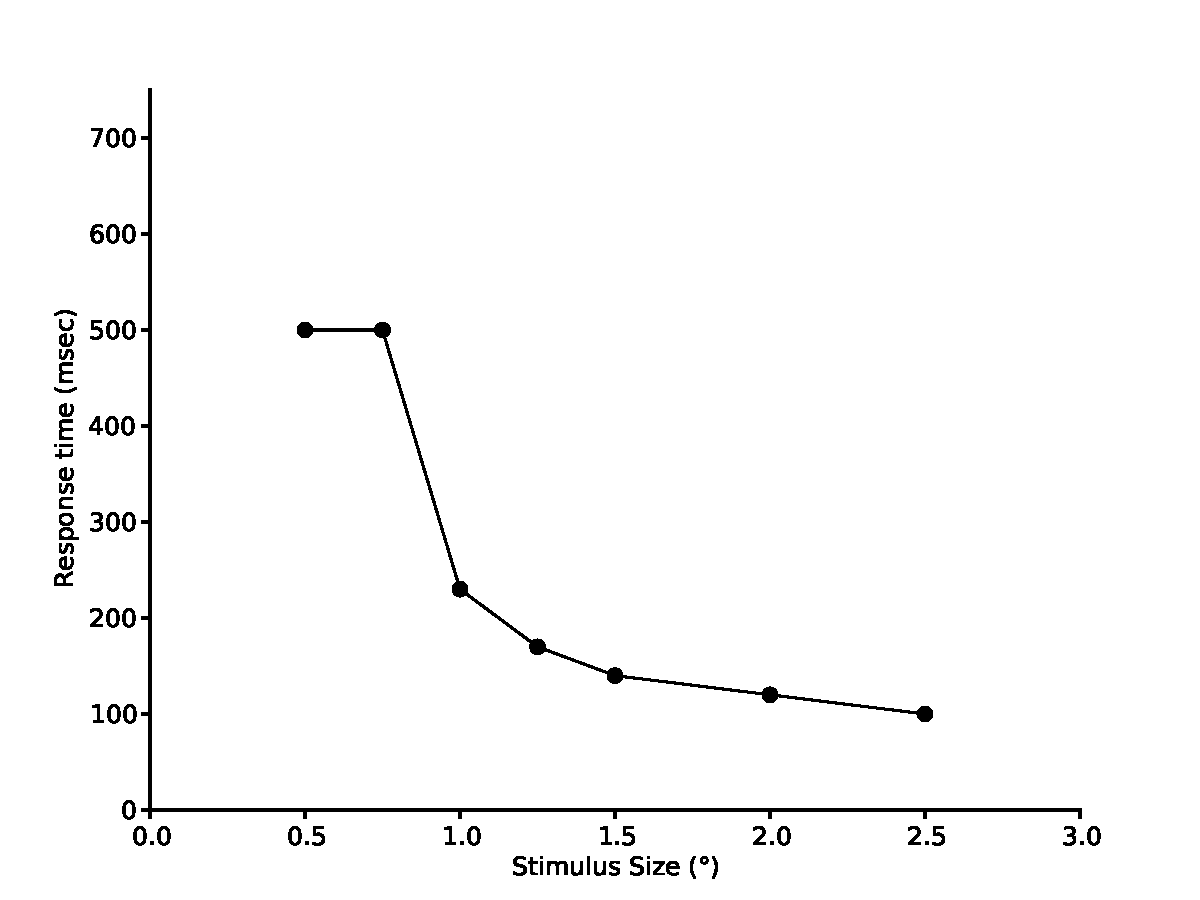
\includegraphics[width=0.5\textwidth]{figures/ch3_7_RT-magnitude-B} \\
    \end{tabular}

  \end{center}

  \caption{Influence de l'excentricité, de la taille et de l'intensité du stimulus sur le temps de réponse. A et B: Le stimulus a été présenté à des excentricités différentes et l'activation a été enregistrée jusqu'à ce qu'elle atteigne la valeur maximale. Le temps de réponse est mesuré quand l'activation atteint le seuil de déclenchement d'une saccade. C et D: Le temps de réponse a été mesuré pour différentes intensités de stimuli (l'intensité de référence vaut 1). E et F: Le temps de réponse a été mesuré pour des stimuli de différentes tailles (la taille de référence vaut 1/90).
  }
  \label{fig: time}
\end{figure}


\subsection{Interactions spatiales entre deux stimuli à excentricités différentes} 


Quand deux (ou plusieurs) stimuli sont présentés sur la rétine, ils activent initialement plusieurs emplacements sur la carte du \gls{sc}. Cependant, après que la carte atteint un état d'activation stable, une seule sous-population d'unités neurales préalablement activées reste active.\\

\begin{figure}
  \begin{center}
      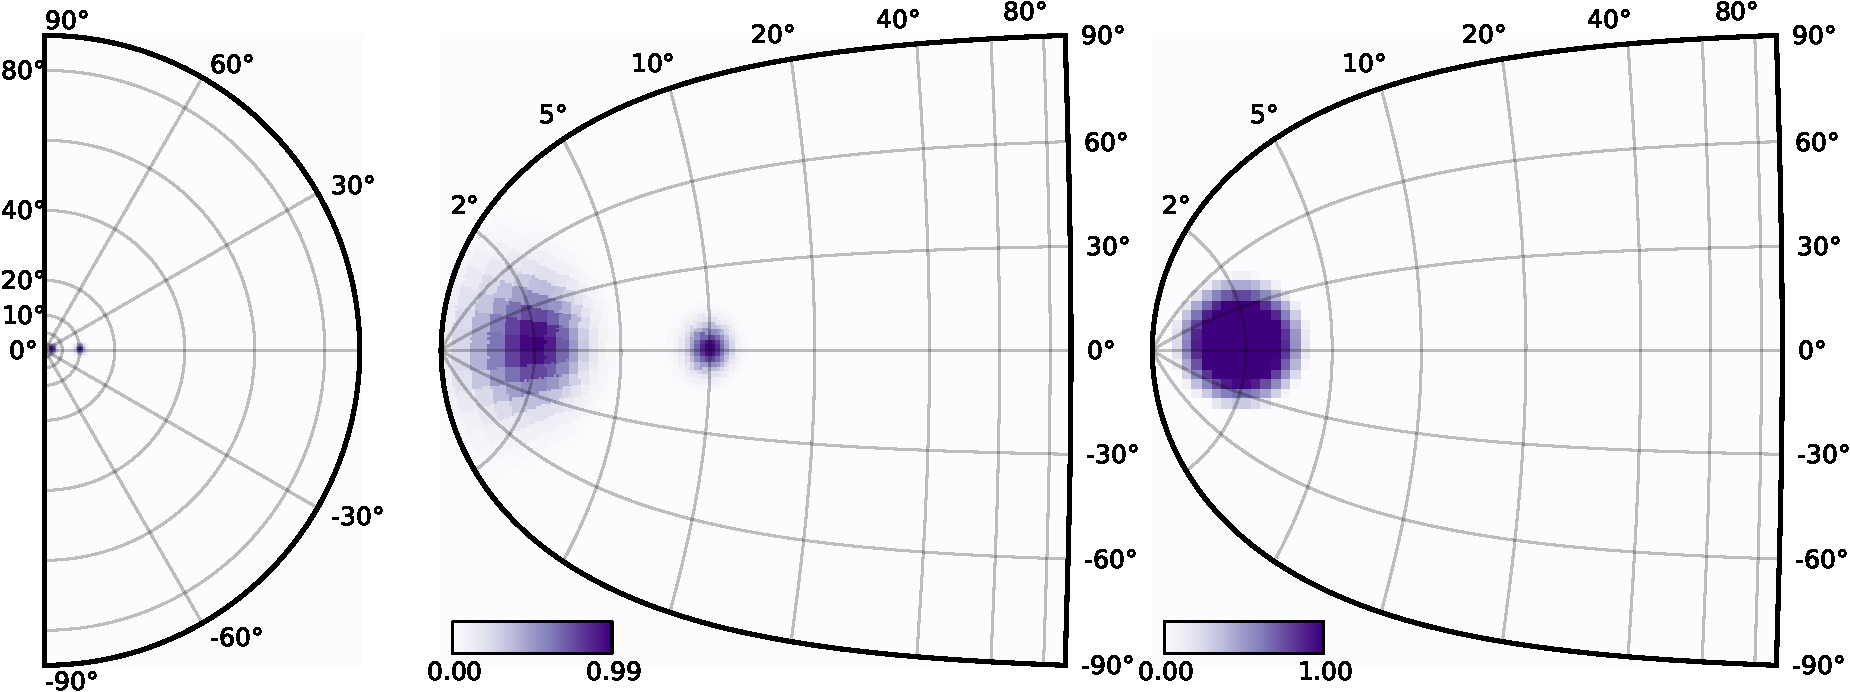
\includegraphics[width=\textwidth]{figures/ch3_8_stimulus-2} 
  \end{center}
  \caption{Interaction spatiale entre deux stimuli identiques à deux positions à même amplitude (0°) et à excentricités différentes (3° et 10°). Le stimulus à 3° active initialement une population plus importante et gagne au final la compétition.
  }
  \label{fig: space}
\end{figure}

 La figure (fig \ref{fig: space}) montre la réponse de notre modèle à la présentation de deux stimuli identiques (même taille, intensité et forme) situés à différents emplacements (3 et 10°). La figure du milieu correspondant à la carte intermédiaire (l'entrée colliculaire suite à la déformation logarithmique) montre que la population activée par le stimulus rostral (3°) est initialement plus grande que la population activée par le stimulus le plus caudal (10°). A la fin de la simulation, figure à droite, l'activité dans le \gls{sc} atteint un état stable et la population active résultante est située dans la position la moins excentré. Le stimulus le plus fovéal a été choisi alors que l'autre a été inhibé sous l'effet de la connectivité latérale.

\subsection{Interactions spatiales entre deux stimuli à excentricités identiques}

Le comportement de sélection a été souvent étudié lorsque deux stimulus sont présentés simultanément avec des excentricités identiques et des amplitudes opposés. La figure \ref{fig: distractor} montre que pour une distance angulaire inférieur à 50° entre les deux cibles, la sous-population résultante des unités neurales actives dans le \gls{sc} est située dans une position intermédiaire entre les deux sites codant l'emplacement de chaque cible, tandis que pour une distance supérieure à 50°, la sous-population active résultante est située à l'un des deux emplacements. Cette sélection est faite quand on ajoute un bruit blanc à l'activité. C'est surtout le phénomène qui est intéressant, la valeur 50° résulte des paramètres choisis et pourrait donc être ajustée.\\

\begin{figure}
  \begin{center}
    \begin{tabular}[t]{c}
     {\textsf {\textbf A}}  \\
      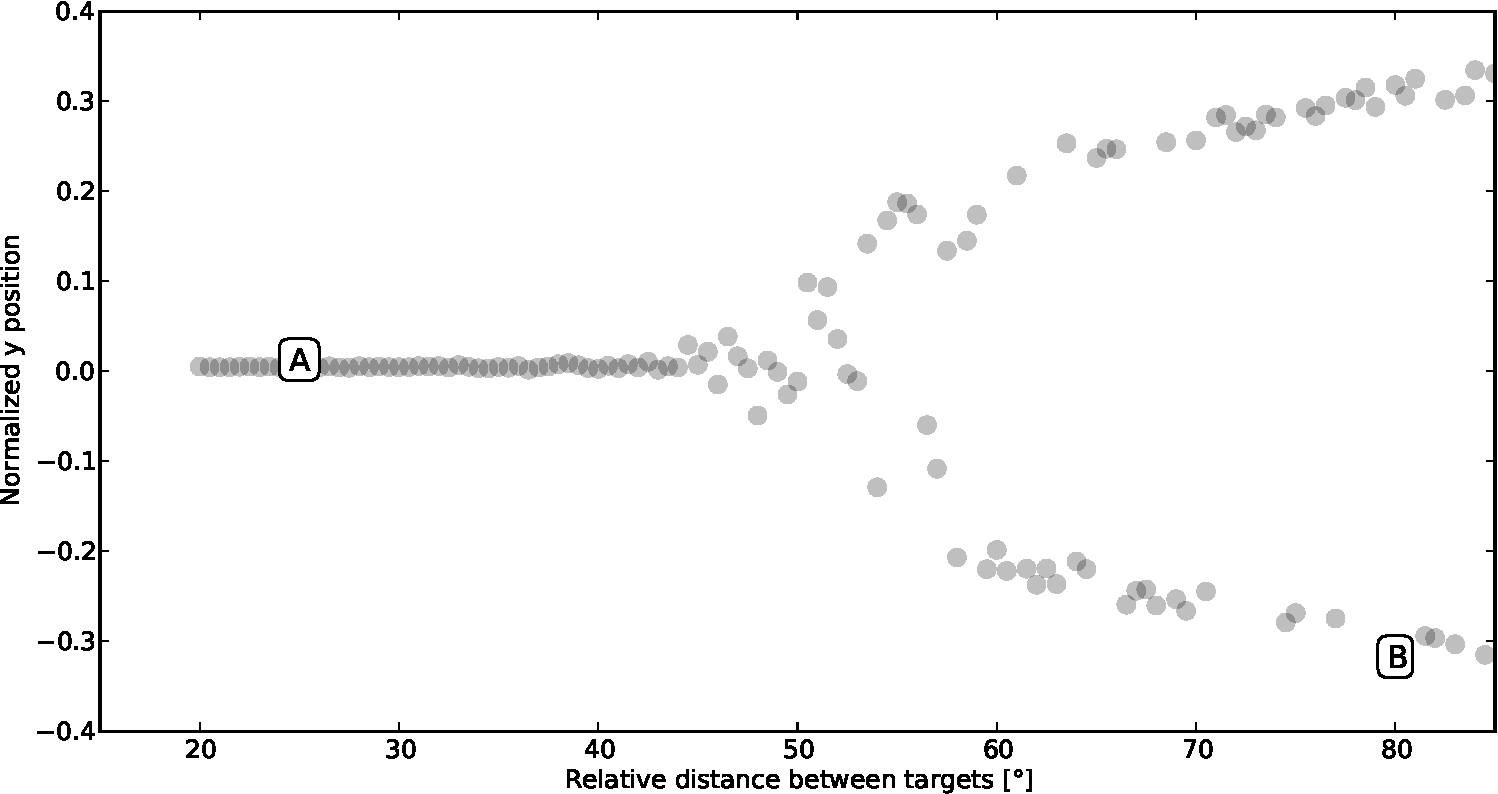
\includegraphics[height=6cm]{figures/ch3_9_global-effect}  \\
    \end{tabular}
    \begin{tabular}[t]{ccc}
      {\textsf {\textbf B}} &
      {\textsf {\textbf C}} &
      {\textsf {\textbf D}} \\     
      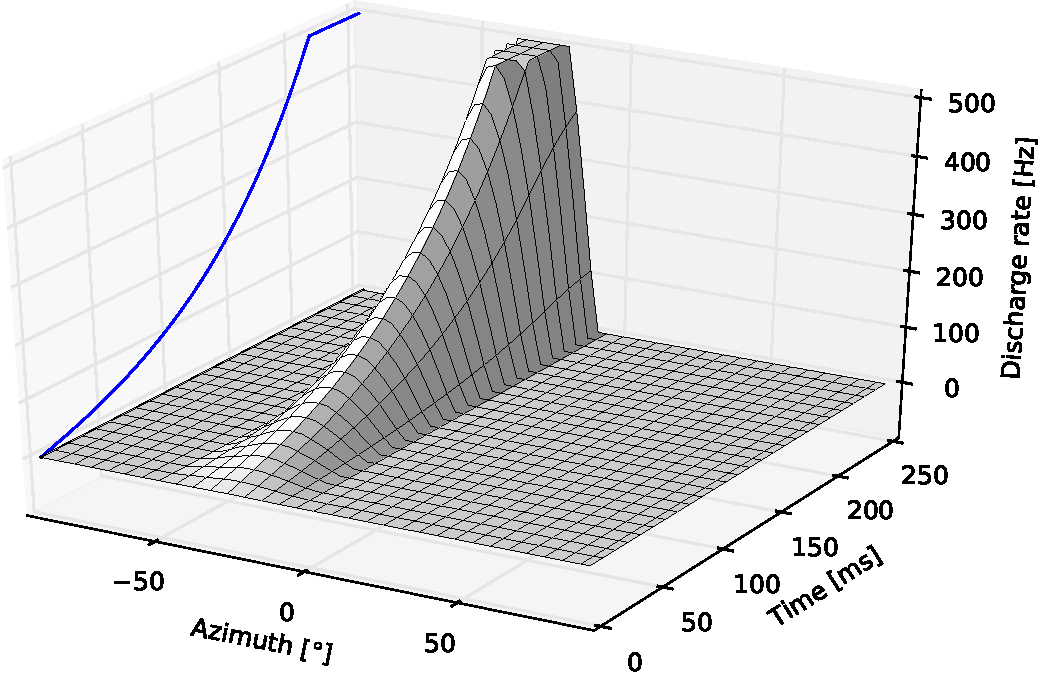
\includegraphics[width=0.33\textwidth, height=6cm]{figures/ch3_9_distractor-effect-1} &
      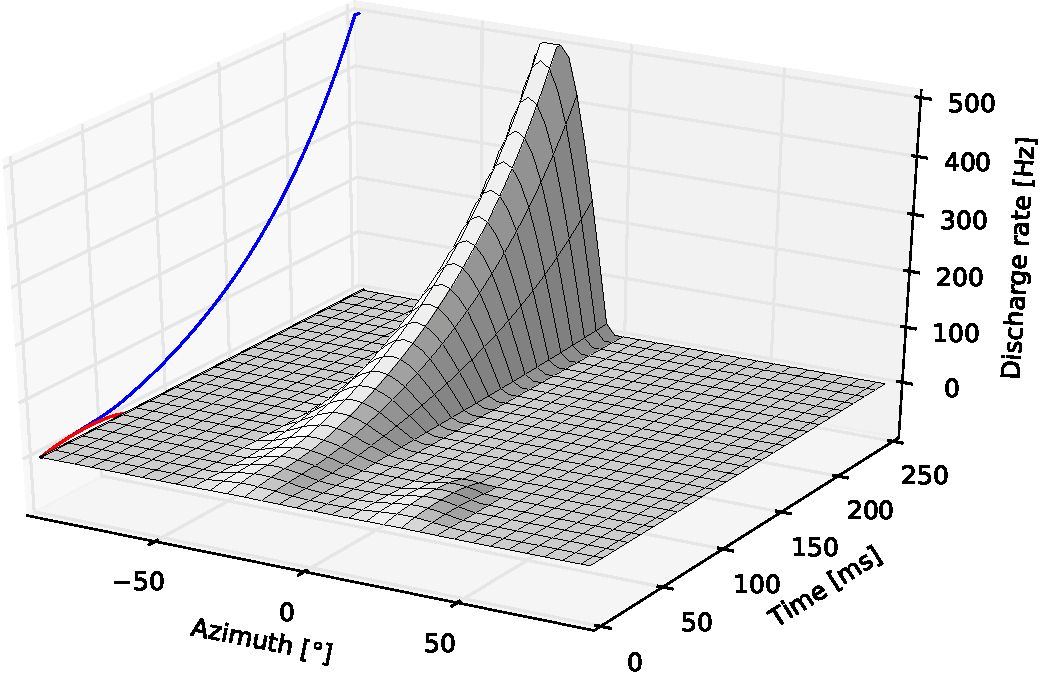
\includegraphics[width=0.33\textwidth, height=6cm]{figures/ch3_9_distractor-effect-2} &
      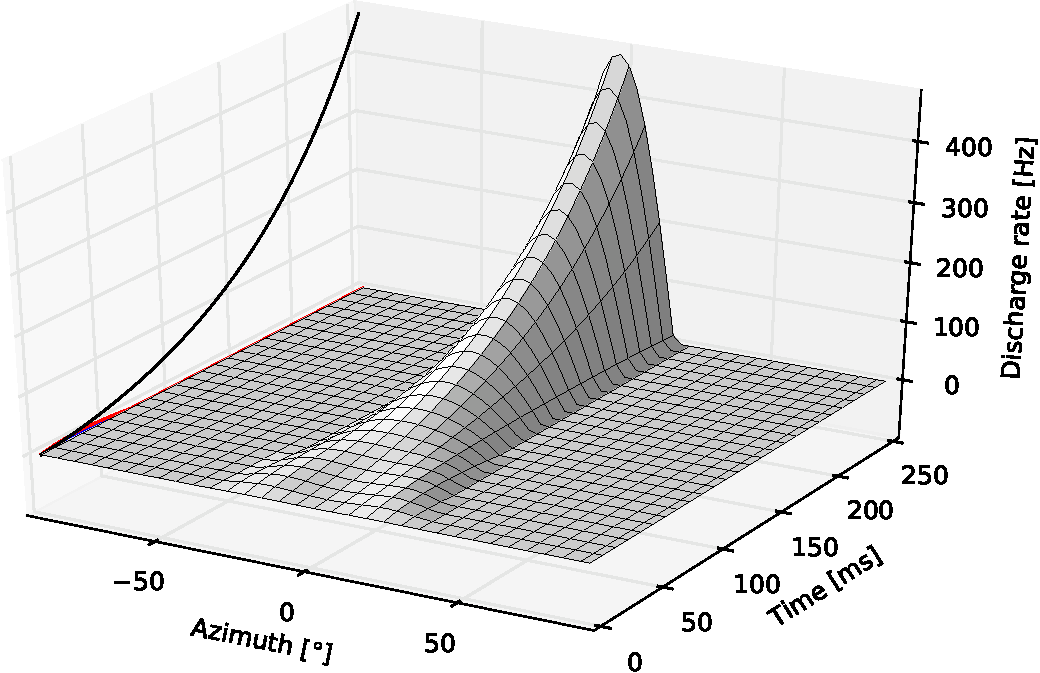
\includegraphics[width=0.33\textwidth, height=6cm]{figures/ch3_9_distractor-effect-3} \\
    \end{tabular}
    \begin{tabular}[t]{cc}
      {\textsf {\textbf E}} &
      {\textsf {\textbf F}} \\     
      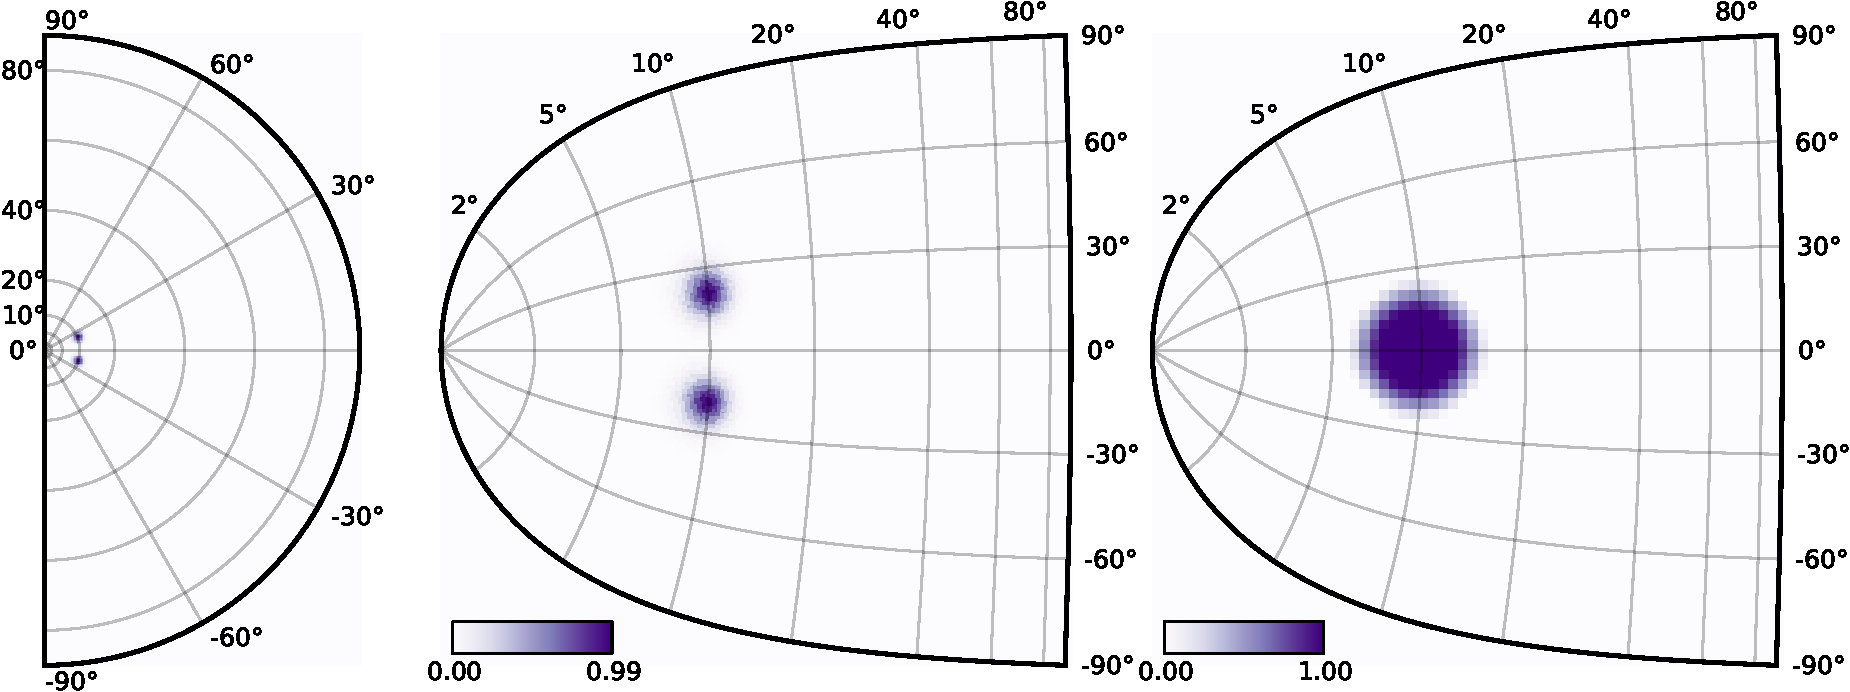
\includegraphics[width=0.5\textwidth]{figures/ch3_9_stimulus-3} &
      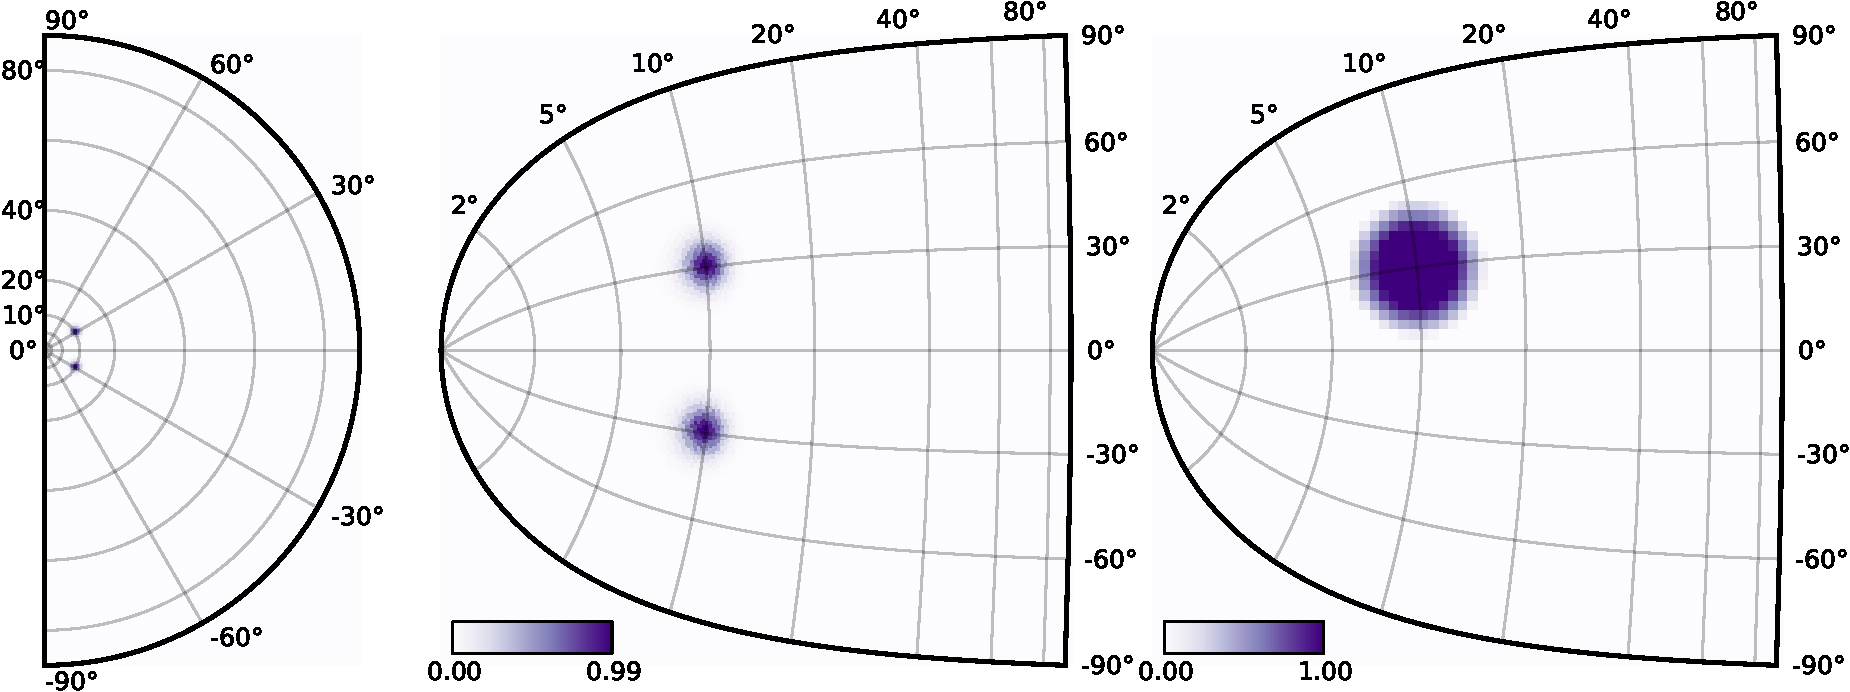
\includegraphics[width=0.5\textwidth]{figures/ch3_9_stimulus-4} \\
    \end{tabular}

  \end{center}

  \caption{Sélection entre deux cibles. A. La position de la cible décodée dans le \protect\gls{sc} après 500ms de simulation. Quand la distance relative entre les deux stimulus est supérieur à 50°, un des deux stimuli est sélectionné. B. L'évolution temporelle de l'activité de la carte du \protect\gls{sc} quand un seul stimuli est présenté. C. L'évolution temporelle de l'activité de la carte du \protect\gls{sc} quand un stimulus est sélectionné. D. L'évolution temporelle de l'activité sur la carte du \protect\gls{sc} montre la fusion des activités au niveau du centre de masse des positions des deux stimuli (pas de sélection). E. L'activation finale du \protect\gls{sc} quand la saccade encodée correspond au centre de masse des deux stimuli (distance relative entre les deux stimuli inférieure à 50°). F. L'activation finale du \protect\gls{sc} quand la saccade encodée correspond à la position de l'un des deux stimuli (distance relative entre les deux stimuli égale à 60°).
  }
  \label{fig: distractor}
\end{figure}


\subsection{Effet de latence}

On peut également examiner l'effet de latence (ralentissement) lors du processus de sélection jusqu'à la stabilisation de l'activité dans la carte colliculaire. Prenons le cas particulier illustré par la figure (fig \ref{fig: distractor}-B et C), quand les deux sous-populations actives ont initialement la même taille (parce que les deux cibles identiques sont à la même excentricité), mais correspondent à des directions opposées. L'évolution de l'activité du \gls{sc} au cours de temps est examinée pour un stimulus simple et comparée à l'activité du colliculus quand ce stimulus est accompagné par un autre stimulus identique à un emplacement symétrique (voir les lignes de projections des courbes (fig \ref{fig: distractor}-B, C et D) en bleu la projection de l'évolution de l'activation maximale causée par le premier stimulus, en rouge celle causée par le deuxième stimulus et en noir l'activation maximale moyenne).

\subsection{Effet de l'inactivation de la carte colliculaire}

Nous avons examiné les effets de l'inactivation d'une petite partie de la carte du \gls{sc}. Dans la figure (fig \ref{fig: accuracy}-B), l'inactivation est imposée sur un site codant une cible située à (5°, 0°). Ensuite, nous avons étudié la réponse du modèle à des stimuli situés à différentes positions. Nous avons constaté que l'activité du \gls{sc} évoquée par les stimuli moins excentrés (4°, 20°) a été décalée vers la partie rostrale du \gls{sc} (correspondant à la projection de la partie fovéale) tandis que l'activité évoquée par une cible plus excentré (9°, - 20°) a été décalée vers l'extrémité caudale (en périphérie). En effet, à cause de l'inactivation, la symétrie de la population, qui est normalement activée pour ces localisations, est changée. La symétrie de l'organisation gaussienne de la connectivité inhibitrice est aussi altérée. La symétrie est rétablie par un décalage de l'activité du \gls{sc} loin du site de la lésion (fig \ref{fig: accuracy}, E, F, G et H). Par contre, un stimulus situé à (5°, 0°) active une population concentrée sur le site inactivé. Enfin, dans la figure, (fig \ref{fig: accuracy}-C), nous montrons l'influence d'une plus grande inactivation utilisant le même stimulus. Certaines des saccades qui n'ont pas été affectées par une petite lésion deviennent inexactes. 

\subsection{Traitement d'images naturelles}

Nous avons également testé le modèle en utilisant des images naturelles issues d'une caméra couleur (CCD). Aucun traitement n'a été réalisé sur l'image, sauf sa transformation en niveaux de gris. La figure (fig. \ref {fig: colliculus}) présente un exemple où une partie d'un clavier d'un ordinateur a été photographiée et introduite au modèle. Cela permet d'illustrer la principale caractéristique du modèle proposé. Si l'on regarde de près la rétine représentant la moitié du clavier (la partie supérieure gauche de la figure), on peut voir que plusieurs lettres ({\tt O, P, L, M} peuvent attirer l'attention et par la suite évoquer une saccade oculaire. Toutefois, la projection rétinotopique sur la carte intermédiaire (V1) du modèle réduit tout naturellement cet ensemble de lettres à {\tt O} et {\tt l}.\\

\begin{figure*}
  \centering
    \includegraphics[width=1.0\textwidth]{figures/ch3_10_colliculus-1}\\
    \includegraphics[width=1.0\textwidth]{figures/ch3_10_colliculus-2}
  \caption{Une image (en couleurs) d'un clavier d'un ordinateur a été prise par une caméra couleur (de résolution $1024 \times 1280$) et transformé en une image en niveaux de gris (normalisés). \textbf{Les figures du haut.} La moitié de droite de l'image a été présentée dans la demi rétine comme entrée de notre modèle. La figure du milieu représente la projection selon l'équation \ref{eq: mapping}. La compétition dans la carte colliculaire fait gagner l'endroit le plus saillant (la lettre {\tt O}) \textbf{Les figures du bas.} Après la saccade, l'image rétinienne est centrée sur la lettre {\tt O}. L'activité colliculaire se concentre alors sur une partie de cette lettre qui semble être l'endroit le plus saillat d'o\`u la position rostrale de l'activation finale de la carte du colliculus.}
  \label{fig: colliculus}
\end{figure*}


Le modèle du \gls{sc} est donc confronté à un choix entre ces deux endroits et la théorie du champ dynamique, comme il a été introduit dans la section précédente, garantit qu'un seul emplacement reste après la compétition. Toutefois, il est difficile de préciser les conditions exactes qui font que le modèle va se concentrer sur la lettre {\tt O} au lieu de la lettre {\tt L} dans l'exemple donné. La forme de la représentation spatiale de la lettre {\tt O} est certainement à prendre en compte.

\section{Discussion}

\subsection{S\'election d'une seule population et stéréotypie des unités neurales actives}

Nous avons constaté que l'état de la carte colliculaire suite à la présentation d'un stimulus visuel se stabilise sur une seule sous-population stéréotypée. Ce résultat est compatible avec les résultats rapportés dans \cite{Anderson:1998}. \cite{Gandhi:2011} ont également évoqué ce phénomène et ont rapporté que la taille de la sous-population des neurones actifs couvre 28\% de la carte juste avant le début de la saccade. Dans l'étude théorique des \glspl{dnf} \cite{Amari:1977}, les auteurs ont montré que pour n'importe quel signal d'entrée constant, l'ensemble des neurones du champ dynamique considéré se stabilise sur une seule sous-population des unités actives avec une forme stéréotypée. Cet effet est dû à l'effet combiné des connexions latérales excitatrices et inhibitrices. \\

L'origine de l'inhibition latérale est un sujet de discussion dans la littérature, correspondant soit à la connectivité intracolliculaire latérale ou à l'inhibition nigrale \cite{Trappenberg:2001} mais dans les deux cas, les modèles supposent que cette inhibition est globale. L'inhibition diffuse assure une compétition dans toute la population neurale du colliculus avec une connectivité latérale excitatrice à effet plus local. Les interactions excitatrices, plus focalisées, créent une boucle de réaction positive, où les unités s'activent les unes les autres. Cette excitation croissante est limitée dans l'amplitude en raison de la non-linéarité de la fonction d'activation et la propagation latérale de l'excitation est limitée par l'anneau de l'inhibition du noyau latéral. Les deux effets ont pour résultat la forme stéréotypée de la sous-population.

\subsection{Explication de la dynamique}

La dynamique de l'activation observée correspond à la relaxation de la stimulation initiale de la carte jusqu'à sa stabilisation. L'état final est une sous-population stéréotypée active. La durée de cette relaxation (temps de réponse) est plus longue quand les états initiaux et finaux de la carte sont plus éloignés. Les états initiaux dépendent de plusieurs paramètres : le nombre de stimuli (discuté ci-dessous), l'intensité et la taille (position et étendue spatiales) des stimulations reçues sur la carte, comme montré dans la figure \ref{fig: time}. \\

%%%%%%%%%%%%%%%%%
Dans \cite {Bell:2006}, les auteurs ont expliqué que la performance dans une tâche de temps de réaction peut être fortement influencée par les propriétés physiques des stimuli utilisés. Plus précisément, ils supposent que un temps de réaction plus court peut être dû à un temps de traitement réduit en fonction de l'intensité du stimulus. \cite {Jaskowki:2004} a également supposé que cette influence peut résulter de la transformation effectuée dans la voie directe de la rétine au colliculus supérieur. \\

%%%%%%%%%%
En outre, les effets de l'inactivation peuvent également être expliqués en se basant sur la dynamique de la population. L'inactivation est une procédure très classique en électrophysiologie et nos résultats correspondent parfaitement aux saccades hypo-métriques et hyper-métriques observées après l'injection de la lidocaïne dans le colliculus supérieur profond \cite{Lee:1988}. En partant de l'activation initiale de la carte colliculaire, la dynamique va tendre à activer une sous-population de taille stéréotypée, permettant ainsi d'avoir une activité stable. La figure \ref{fig: accuracy} montre que cette activation finale est obtenue en décalant l'activation loin du site inactivé, causant alors une inexactitude dans la saccade suivante. Comme on peut observer sur la figure \ref{fig: accuracy}, le décalage se produit dans la direction opposée à la position de la partie inactivée de la population stimulée impliquant les caractéristiques hypo-métriques et hyper-métriques évoquées ci-dessus. \\

Enfin, l'effet montré dans la figure \ref{fig: accuracy}-C est moins intuitif, puisque nous avons expliqué que quelle que soit la taille du stimulus, la sous-population active résultante est stéréotypée. Les figures \ref{fig: accuracy}-B et \ref{fig: accuracy}-C montrent que l'inexactitude provoquée par une inactivation locale dépend de la taille du stimulus. Puisque le décalage de l'activité se produit pendant l'évolution de l'activation de la carte et non pas seulement à la fin, on peut déduire que la stimulation initiale (qui dépend de la taille du stimulus) peut modifier le décalage. Considérons dans la figure \ref{fig: accuracy}-C les saccades qui n'ont pas été affectées dans la première simulation (fig.\ref{fig: accuracy}-B) (loin du site de la lésion), un plus grand stimulus active initialement une plus grande population dans le \gls{sc}. Alors l'inactivation cause une asymétrie dans l'activation d'entrée et pousse le décalage de l'activité loin du site de la lésion.


\subsection{Effet de la projection logarithmique}

Comme expliqué ci-dessus, pour des caractéristiques semblables et en raison de la projection logarithmique, une cible moins excentré implique en entrée l'activation d'une plus grande sous-population qui atteindra par conséquent le profil standard d'équilibre moins rapidement. En effet, la compétition est plus lente et le système prend plus de temps pour se stabiliser.\\ %et ceci est en accord avec le fait que la latence  augmente avec l'amplitude de la saccade comme montrée par \cite{Goossens:2006}.\\
%%%%
La projection logarithmique qui amplifie la représentation de la région rostrale explique également la largeur croissante des champs récepteurs (courbes d'accord) comme le montre la figure \ref{fig: time} et explique également leur asymétrie. Ces courbes d'accord correspondent bien aux propriétés du champ de mouvement décrites dans les résultats expérimentaux de \cite{Munoz:1995a, Sparks:1976}. \\

Comme signalé dans \cite{Sparks:1980}, chaque unité colliculaire atteint son activation maximale en réponse à une direction et une amplitude particulières, indépendamment de la position initiale de l'oeil dans son orbite. D'ailleurs, l'activation est de moins en moins importante pour les directions voisines en s'éloignant de l'emplacement préféré et disparaît pour les saccades vers des emplacements qui sont très loin de l'emplacement préféré. La nature asymétrique des champs récepteurs peut également expliquer les petites erreurs dans l'exactitude (fig.\ref{fig: accuracy}): des saccades hypo-métriques (respectivement hyper-métriques) vers les stimuli rostraux (respectivement caudaux). Il y a aussi de telles erreurs aux bords de la carte colliculaire mais dans ce cas le problème vient aussi du fait qu'on a considéré un seul hémichamp. En effet, quand les deux hémichamps visuels sont considérés, les régions latérales sont associées à une activation bilatérale, par les deux colliculi.


\subsection{Interaction entre plusieurs stimulus}

Plusieurs études ont fourni des données sur l'organisation du chemin saccadique que les sujets suivent quand ils explorent des images \cite{Yarbus:1967, Noton:1971, Levy:1974}. Elles ont prouvé que la valeur attractive d'un objet dépend fortement de sa distance relativement à l'objet fixé précédemment. Cette valeur attractive est plus importante quand l'objet est plus proche, donc sa projection est plus fovéale. Notre modèle reproduit des réponses semblables quand plusieurs objets sont présentés (fig.\ref{fig: space}).\\

Nous avons expliqué qu'à cause de la transformation log-polaire, deux stimuli visuels de tailles semblables activent deux populations avec des tailles qui dépendent de leurs excentricités : Une sous-population plus grande est activée quand le stimulus est projeté près de la région fovéale (fig.\ref{fig: space}). Nous avons également constaté que la dynamique de l'activité colliculaire assure une fonction de type ``le gagnant prend tout'' (\textit{winner-takes-all}) résultant de la théorie des \glspl{dnf}. Indépendamment de l'emplacement des stimuli, à la fin de chaque simulation une seule cible est choisie.\\

Néanmoins, prendre une décision peut durer plus ou moins longtemps pour atteindre le profil standard d'activation selon l'état initial. Quand deux sous-populations éloignées sont activées initialement (dans le cas de deux stimuli), elles entrent en compétition par leurs connexions inhibitrices à longue portée. La population initialement plus grande (en étant plus rostrale par exemple) aura plus de puissance à inhiber l'autre et donc atteindre l'état final stable et gagner la compétition, comme on l'a expérimentalement observé dans la section précédente (fig.\ref{fig: space}).\\

L'effet du distracteur distant (\textit{remote distractor effect}) a été examiné pour la première fois par \cite{Levy-Schoen:1969} dans une étude où l'auteur a essayé de découvrir ``les règles'' qui régissent le mécanisme de sélection d'une cible visuelle. Dans cette étude, deux stimuli identiques ont été simultanément présentés à deux emplacements différents afin d'examiner le processus de sélection. Nous proposons ici que la sélection du stimulus le plus rostral résulte directement de l'effet de la connectivité latérale (excitatrice et inhibitrice) dans une carte du \gls{sc} d'une part et de la représentation géométrique du champ visuel qui amplifie la représentation des régions proches de la fovéa. 
%%%%%%%%%%%%%%%%%%%%%%%%%%%%

\subsection{Dynamique temporelle pendant la compétition}

Un effet de latence ralentissant le processus de sélection entre deux stimuli est rapporté dans plusieurs études \cite{Findlay:1983, Weber:1994, Godijn:2002, Honda:2005} utilisant plusieurs scénarios (différents emplacements, différentes synchronisations entre les présentations des deux stimuli). Nous avons reproduit certaines de ces expériences en utilisant le modèle proposé pour étudier l'effet de latence évoqué par la présence d'un distracteur. Comme expliqué ci-dessus, la compétition entre les bulles d'activités prend un certain temps avant qu'une sous-population s'inhibe et son activité disparaisse permettant d'atteindre le profil stéréotypé.\\

Nous avons étudié le cas o\`u les deux stimuli sont à la même excentricité et activent le même nombre d'unités (fig \ref{fig: distractor}-C). Pendant les premières 25ms qui suivent la présentation des stimulus, les deux emplacements correspondants dans la carte du \gls{sc} sont stimulés et chaque sous-population d'unités actives tend à empêcher l'autre sous-population par les connexions inhibitrices à longue portée. Cette compétition pourrait théoriquement durer jusqu'à la disparition des stimuli si le système était parfaitement symétrique et non-bruité. Puisque nous appliquons un bruit blanc aléatoire au niveau de la rétine, le bruit perturbe la symétrie et favorise un des deux emplacements, menant à la sélection finale.\\

Dans ce cas, avec une distance angulaire entre les stimuli de 60°, les connexions inhibitrices à longue portée assurent une compétition entre sous-population actives avant de choisir la cible (fig.\ref{fig: distractor}-F). Dans une étude plus systématique, on montre sur la figure \ref{fig: distractor}-A que pour des distances angulaires plus courtes (la limite étant évaluée ici à 50°), la sous-population active résultante est située au milieu des deux emplacements comme dans l'exemple de la figure \ref{fig: distractor}-D, on parle alors d'un ``effet global''. \\

L'effet global a été d'abord rapporté dans \cite{Coren:1972} pour les saccades volontaires et plus tard confirmé pour toutes les saccades vers des cibles visuelles \cite{Deubel:1984, Findlay:1982} et récemment pour les distracteurs \cite{VanderStigchel:2011}. Il s'agit du cas o\`u deux stimuli sont présentés à des emplacements proches dans l'espace, la saccade résultante est dirigée vers un emplacement intermédiaire, fortement corrélé avec le centre de gravité des deux emplacements de stimuli. Quand les sous-populations initialement activées par les deux stimuli sont proches (interfèrent), non seulement les inhibitions à longue portée mais également les connexions excitatrices à courte portée vont agir mutuellement sur les sous-populations de neurones. Le processus d'excitation a un effet constructif qui permet de recruter une sous-population moyenne (le plus probablement à leur centre de masse). Donc une nouvelle activation évolue jusqu'au atteindre le profil standard et déclenche la saccade (fig.\ref{fig: distractor}-D). Ces résultats relatifs à l'effet global sont intéressants parce qu'il n'y a pas besoin d'ajouter un mécanisme de choix puisque la sélection de cible résulte simplement de la connectivité latérale. 


\section{Conclusion}

En conclusion, de nombreuses propriétés locales du colliculus supérieur peuvent être expliquées en termes d'émergence résultant simplement de la dynamique interne entre les neurones du \gls{sc} et la projection logarithmique. En d'autres termes, le modèle est, d'une part, basé sur une règle bio-inspirée de fonctionnement local et homogène, d'autre part, lié avec le monde extérieur à travers un flux d'informations provenant de la rétine. Il en résulte deux conséquences. D'abord, le modèle proposé peut représenter une base solide pour les travaux futurs qui visent à modéliser la boucle visuo-motrice. Ensuite, ce modèle suggère clairement que la plupart des expériences mesurent réellement les mêmes propriétés de bas niveau qui peuvent différer seulement dans leurs expressions comportementales.\\

La validation des résultats des simulations du modèle et sa justification par rapport aux données biologiques ont été faites en collaboration avec des collègues des neurosciences. Nous n'avons pas présenté ici des expériences qui permettent de proposer des prédictions et d'inspirer en retour les biologistes pour effectuer des expériences supplémentaires. Nous travaillons le sujet avec des collègues biologistes. En particulier, la dynamique de notre modèle prédit que l'augmentation de la taille du stimulus dans le cas de l'inhibition locale cause un élargissement de la zone d'altération des saccades. A notre connaissance, l'expérience n'a pas été encore été faite. Nous sommes aussi en train d'examiner la réponse du modèle à différentes formes géométriques de stimuli.\\


En résumé, nous avons considéré dans notre modèle un traitement en feed-forward (séquentiel) des entrées exogènes provenant de la rétine, basé sur des règles locales simples dans une population homogène. Ce modèle nous a permis d'expliquer plusieurs résultats biologiques et comportements du système oculomoteur sans tenir compte des contributions endogènes de transport des informations telles que les instructions, les objectifs ou les motivations provenant des autres structures nerveuses. Il serait donc pertinent de considérer ces contributions pour mettre en oeuvre des comportements plus complexes.\\

En effet, si on revient sur l'exemple de l'image réelle, on peut estimer la difficulté inhérente à l'organisation temporelle de l'enchaînement de saccades oculaires en l'absence d'un contrôle de haut niveau. Si nous devions laisser le modèle réagir tout seul avec son environnement, il aura certainement tendance à se concentrer sur l'emplacement le plus saillant, sans jamais explorer d'autres points d'intérêt (d'un point de vue comportemental). Une fois qu'une saccade est programmée et réalisée, la saccade suivante doit se diriger vers un nouvel endroit saillant. Le modèle recruterait donc une nouvelle sous-population colliculaire codant le nouvel emplacement à condition d'inhiber la région fovéale (activée par la présence du stimulus fixé suite à l'ancienne saccade) pour éviter que le modèle ne reste coincé sur cet endroit. Mais dans un tel cas, rien n'empêcherait le modèle de se piéger dans un cycle d'allers retours entre les deux endroits les plus saillants. Pour explorer toute la scène visuelle, il faut donc une sorte de contrôle extérieur pour pouvoir inhiber par exemple les activations correspondant à des endroits déjà ciblés pour favoriser d'autres endroits \cite {Fix:2006} ou bien porter l'attention plutôt sur les endroits les moins saillants en ajoutant la notion de la motivation. On s'intéressera à ce dernier point dans le chapitre suivant en introduisant la notion de sélection motivée à travers un modèle qui porte sur le rôle des ganglions de la base dans la sélection.\\


